\documentclass[
  final,
  babelLanguage=british,
  %desktopVersion,
  %showtrims,
  %overleaf,
]{anecdote}

%\graphicspath{{./assets/photos/300dpi/}}
\graphicspath{{./assets/photos/92dpi/}}

% Page size: 5.25 x 8 inch
% Body text: 11 / 16 pt

\usepackage{local}

%% Details of the book
%% ===================

\title{Alert to the Needs of the Journey}
\subtitle{}
\author{Ajahn Munindo}
\publisher{Aruno Publications}
\date{2017-12-06}
\editionInfo{\textit{First edition}, printed in Great Britain, 2018}
\ISBN{978-1-908444-61-5}

% === Metadata ===

\hypersetup{
  pdftitle={\thetitle},
  pdfauthor={\theauthor},
  pdfcopyright={Copyright (C) 2018, \thePublisher},
  pdfsubject={Dhamma talks by Ajahn Munindo},
  pdfkeywords={buddhism, dhamma},
  pdflicenseurl={https://creativecommons.org/licenses/by-nc-nd/4.0/},
  pdfcontacturl={https://ratanagiri.org.uk},
  pdflang={en},
}

\pdfinfo{
  /Title (\thetitle)
  /Author (\theauthor)
  /Subject (Dhamma talks by Ajahn Munindo)
  /Keywords (buddhism, dhamma)
  /GTS_PDFXVersion (PDF/X-1:2001)
  /GTS_PDFXConformance (PDF/X-1a:2001)
}

%% === Load further packages ===

%% === Hyphenation exceptions and corrections ===

\hyphenation{London knowing Citta-viveka}

\begin{document}

\frontmatter

\ifdesktopversion
\desktopCover{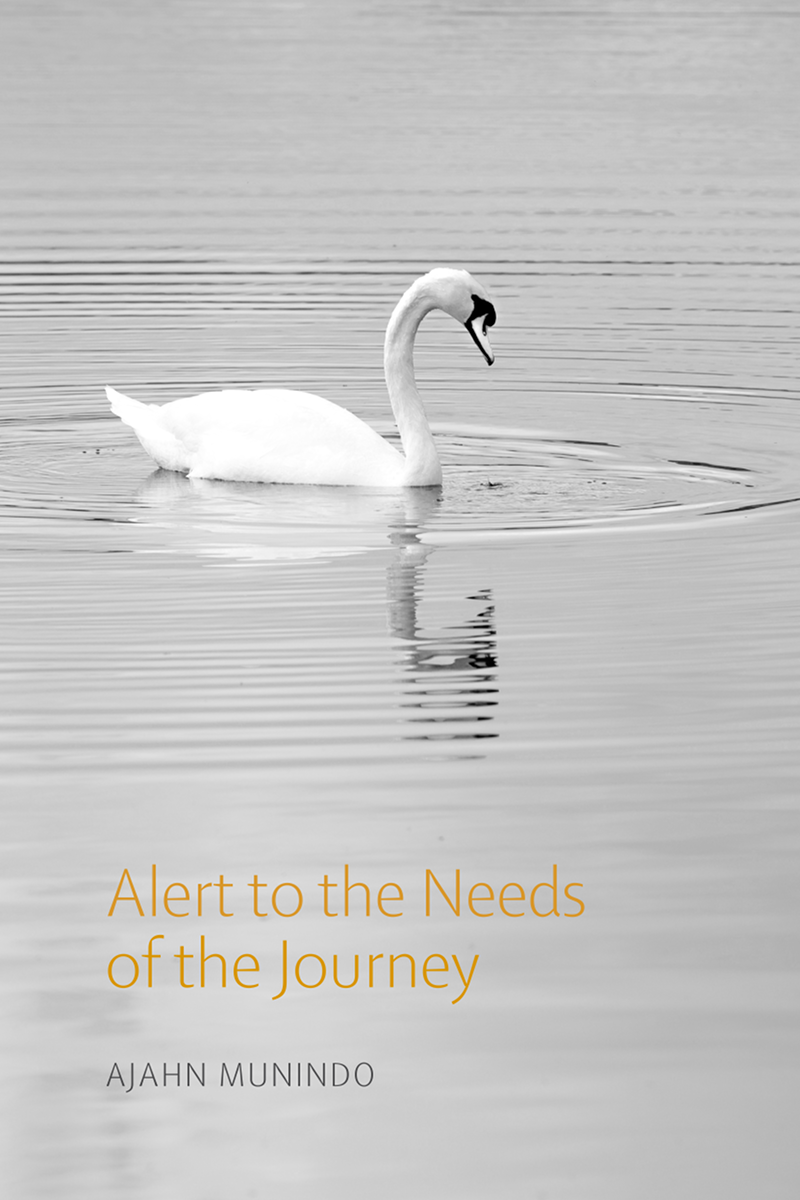
\includegraphics[height=\paperheight]{./desktop-cover.png}}
\else

\thispagestyle{empty}
\mbox{}
\pagecolor{frontyellow}
\newpage
\thispagestyle{empty}
\pagecolor{white}
\mbox{}
\newpage

\fi

\cleartorecto
\thispagestyle{empty}

\mbox{}\vfill

{\raggedright
\itshape
Alert to the needs of the journey,\\
those on the path of awareness,\\
like swans, glide on,\\
leaving behind their former resting places.

Dhammapada 91\par}

\vfill\mbox{}

\cleartorecto
\thispagestyle{empty}
\vspace*{5em}

{\centering

\settowidth{\titleLength}{%
  {\Large\chapterTitleFont\scshape\MakeLowercase{\thetitle}}%
}

{\Large\chapterTitleFont\scshape\MakeLowercase{\thetitle}}\\[0.3\baselineskip]
\setlength{\xheight}{\heightof{X}}
\raisebox{0.5\xheight}{\color[gray]{0.4}\rule{\titleLength}{0.25pt}}\\[0.3\baselineskip]
{\itshape
\thesubtitle}

\vfill

\theauthor

\vspace*{5em}

}



\cleartoverso
\thispagestyle{empty}

{\copyrightsize
\raggedright
\setlength{\parindent}{0pt}%
\setlength{\parskip}{0.8\baselineskip}%

\thetitle\\
by \theauthor

This publication is made available\\
for free distribution\\
by Aruno Publications

Aruno Publications is administered by:\\
Harnham Buddhist Monastery Trust\\
Company No. 6688355,\\
Unincorporated Charity Reg. No. 1126476

Contact Aruno Publications at \href{https://ratanagiri.org.uk/}{www.ratanagiri.org.uk}\\
This book is available for free download at\\
\href{https://forestsangha.org/}{www.forestsangha.org}

ISBN \theISBN

Copyright \copyright\ Aruno Publications 2018

\vfill

{\footnotesize

This work is licensed under a Creative Commons\\
Attribution-NonCommercial-NoDerivatives 4.0 International~License.

Produced with the \LaTeX\ typesetting system, set in Gentium, Shaker,\\
Merriweather and Hattori Hanzo.

\theEditionInfo

}}


\cleartorecto
\tableofcontents*

\chapterTitleVertical{I\\N\\T\\R\\O\\D\\U\\C\\T\\I\\O\\N}

\chapter{Introduction}

TODO


% Page 1 is the first page of the first chapter.
\mainmatter

\chapterNote{%
Alert to the needs of the journey,\\
those on the path of awareness,\\
like swans, glide on,\\
leaving behind their former resting places.

Dhammapada 91}

\chapterTitleVertical{K\\E\\E\\P\par M\\O\\V\\I\\N\\G\par O\\N}

\chapter{Keep Moving On}

\tocChapterNote{Dhammapada 91, letting go, faith, Heartwood sutta, integrity,
fear, desire, honesty, consistency, ascetic practices, addictions, agility.}

Let us consider together this short teaching from the Buddha.

When we begin on this journey we are all seeking, in some form or
another, an increased sense of freedom. Maybe we were motivated by an
altruistic vision of living with greater compassion. Or perhaps it was
the clarity and detail of the Buddha’s analysis of the human mind that
inspired us. For many it was maybe just a matter of trying to find
relief from the burden of suffering. Whatever it was that brought us to
the beginning of this path, we all benefit from the encouragement
offered by those who have travelled ahead of us.

Here, in this Dhammapada verse 91,\cite{dhammapada-aruno}
the Buddha is pointing out the
benefit of cultivating a willingness to keep beginning again in our
practice. He doesn’t want us to settle anywhere short of realizing the
goal of freedom. He wants us to keep practising whatever happens.

When we start out we can’t know what the journey will be like. There
will be periods of gladness and possibly periods of sadness. Sometimes
we will feel as if we are making progress, and at other times we might
feel thoroughly stuck. At times we will feel confident, and at other
times we might feel as if we are sinking in a swamp of doubt. The Buddha
encourages us not to settle anywhere, but to keep letting go until the
wisdom that knows the way to freedom becomes perfectly clear.

\section{Training to See with Insight}

Fortunately for us, throughout the centuries this Theravada Buddhist
tradition has maintained tried and tested teachings on the cultivation
of letting go in the pursuit of wisdom. The teachers and the tradition
are still readily available to offer us guidance. And there will
definitely be times in our training when we need that guidance.

There is a word in the Pali language that we recite in our chanting when
describing the qualities of the Buddha: \emph{lokavidu}, which means ‘one who
knows the world’. ‘Knowing’ here refers to a direct, transformative kind
of knowing. It is not the knowing with which we are generally familiar,
a knowing \emph{about} things. This path of practice is characterised not by
what we learn about on it, but by the effort we make to develop a fresh,
new way of seeing.

When we say \emph{Dhammaṃ saraṇaṃ gacchāmi}, ‘I go for refuge to the Dhamma’,
we are saying that more than anything else we are interested in seeing
the reality of the world. Here the world is not just the outer world,
but the inner worlds too, all that we create in our minds. Being a
knower of the world means knowing the truth of gladness and sadness,
confidence and doubt, liking and disliking – and being able to accord
with this truth; being at peace with it. There is no limit to the
information we can accumulate about the world, but now we are learning
to see what the world looks like when we have let go of habits of
clinging. We are training to see with insight.

\section{Not Believing}

There will be times when we feel love and gratitude towards our teachers
and the tradition, and probably there will be times when we don’t. I
spent the early years of my monastic training, most of the period
between 1976 and 1979, at Wat Pah Nanachat in NE Thailand. I recall
first arriving there and feeling filled with gratitude; there was a
tremendous sense of relief. At last I was somewhere I truly wanted to
be. I didn’t want to be anywhere else in this whole wide world, and I
felt privileged to be received into that community. The monastery had
only been established for a few months. To say food and accommodation
were basic is an understatement, but the grass-roof huts and the modest
one meal a day were just wonderful. To be in the company of the radiant
and gracious Ajahn Sumedho and his fellow Western wayfarers was a source
of joy and inspiration.

I can also vividly recall wondering months later what it would be like
if only I could escape from this hell-hole. One morning, as we walked on
alms-round and crossed over some railway tracks, I stopped for a few
moments to feel the tracks beneath my bare feet, and imagined how those
railway lines went all the way to Bangkok, and how perhaps there I could
be relieved from the intense misery I was having to endure. It can be
difficult to release ourselves from the momentum we have generated by
following the habit of believing in our moods, including both agreeable
and disagreeable moods. Thankfully on that occasion in my training I
didn’t completely believe in what the mood was telling me, otherwise I
would have given up.

Whether we love our teachers and our tradition or not, what training in
insight is about is learning to let go of the way things appear to be,
to stop merely believing and see that which is true. When we see
accurately, we arrive at a true appreciation of whatever there is in
front of us, be it our teachers, our moods or anything else. We won’t
have to be driven by conditioned liking and disliking, and that means we
won’t get stuck. All this conditioned activity of liking and disliking
is what is meant by the world. Insight sees through the world, revealing
its instability and the fruitlessness of our habits of clinging. Wisdom
sees how the clinging creates resistance and causes suffering. The
warm-hearted expression of such wisdom is compassion.

\section{Becoming Stuck}

The Buddha doesn’t want us to settle too soon, but to keep moving on
until we arrive at real wisdom and compassion. It is because of
unawareness regarding the truth of our preferences – our liking and
disliking – that our view of the world is distorted. Having preferences
is not wrong per se; it is the way we have them which makes the
difference. The untrained mind is regularly fooled by the way things
appear to be. The Awakened Ones are never fooled, hence they never
suffer.

Before his enlightenment the Buddha-to-be was also lost in liking and
disliking, he too was fooled by the way the world appeared to be and
suffered accordingly. When he felt happy he believed ‘I am happy’. When
he felt sad, he believed ‘I am sad’. But eventually, growing tired of
the mediocrity of such an existence, he set out in search of a solution.
He trained his inner spiritual faculties to the point where eventually
he could see beyond all the conditioned activity of mind, beyond the
‘world’, to what he referred to as the unconditioned. From that point
onward he knew directly that whatever conditions arose in his mind, they
were simply passing through. Nothing could get stuck. He was fully freed
and fully available to bring benefit into the world.

The Awakened Ones view all existence according to what is real.
Unawakened beings see according to what we project onto the world by way
of our preferences. Every time we attach to something, we become stuck
there for a while. If we are training rightly, we gradually learn to
recognize sooner what we are doing. If we want to measure our progress
in practice, it should be in terms of how long it takes us to remember
that we are doing the clinging, we are doing the suffering; it is not
something external that is happening to us. Whether gross or refined,
the same principle applies.

\section{The Discourse on the Heartwood}

One reason for emphasizing the importance of establishing practice on
the principle of beginning again, over and over, is because the
temptation to settle, to get stuck, can arise at any stage. We don’t
only need to be careful about our coarse fluctuating moods. It is also
possible to become stuck in refined levels of concentration.

My first meditation teacher in Thailand, Ajahn Thate\cite{ajahn-thate}
was very adept
at abiding in highly refined states of samādhi. He relates how he spent
ten years stuck in unproductive states of tranquillity. It took the
penetrative insight and helpful support of Ajahn Mun to guide him away
from his fondness for samādhi and, by establishing his meditation in
body contemplation, to proceed towards awakening.

Some of you will be familiar with the discourse by the Buddha known as
the \emph{Mahā-sāropama Sutta},\cite{mahasaropama-sutta}
the Discourse on the Simile of the Heartwood.
In this teaching the Buddha likens someone setting out in
pursuit of awakening to someone going in search of heartwood, the most
valuable portion of a tree. Initially spiritual aspirants trust that
reaching the goal is possible and are energized into making an effort.
However, quite quickly they find that just being on the spiritual
journey means they gain increased respect; their status in society
rises, and they decide this level of increased well-being is good enough
and cease making efforts. The Buddha likens this to someone setting out
in search of the heartwood but settling for a bunch of twigs. In other
words, if we find ourselves feeling pleased with the praise we receive,
for having impressed a few friends with our spiritual efforts, that is
not the place to get comfortable.

The discourse goes on by likening the aspirant who settles for the level
of elevated ease and contentment which comes with upgraded integrity to
someone settling for a portion of the outer bark of a tree. Then the
seeker who grows comfortable with the increased well-being which comes
with concentration and tranquillity is likened to someone going away
with a portion of the inner bark. Resting at the level of initial
insight is likened to the seeker becoming contented with a portion of
the sapwood. It is not until full awakening is reached that the Buddha
says the seeker has arrived at the heartwood.

\section{Beginning Again}

At any stage of practice we can be fooled into believing that ‘this is
good enough’ and abandon making efforts. We manage the risk of this
happening in advance by cultivating the wholesome habit of willingly
beginning again. This doesn’t mean we never rest or pause to delight in
the increased sense of freedom which comes from letting go. Certainly,
taking all the time we need to regularly refresh and renew our body and
mind is skilful – so long as a pause doesn’t turn into a fixed position.
The pleasure that comes with receiving praise and popularity, for
instance, can be intoxicating. Or perhaps the more subtle pleasure that
comes from samādhi could tempt you to settle. Maybe you feel it’s time
to start sharing your wisdom and compassion with the world, and set up
your own YouTube channel. But if you feel it is ‘my’ wisdom and
compassion, it would definitely be better to ‘keep moving on, leaving
behind former resting places’.

And it is not only our own increased ability that might distract us from
the path; we could become blinded by somebody else’s aura. There are
many teachers around looking for disciples, and if they catch us in
their spotlight we can lose perspective. Allowing ourselves to become
overly impressed by stories about the magic powers and super-abilities
of others, however noble they are, does not necessary bring benefit. As
the Buddha advised in
the \emph{Mahā-Maṅgala Sutta},\cite{mahamangala-sutta}
we can learn from ‘association with the wise’, but if we are truly learning, we will keep
letting go.

\section{Clumsy Beginnings}

Our ability to keep moving on is not always going to feel comfortable.
We won’t automatically start out with an ability to glide on smoothly.
Especially early on, our excessive enthusiasm can cause our efforts to
be somewhat clumsy. When I was living under Ajahn Chah, there was an
occasion when I was called upon to translate for a newly arrived novice.
This eager young man wanted Ajahn Chah’s advice on how he should set up
his practice during the approaching Rains Retreat (\emph{vassa}). He
explained that he was determined to practise really hard and intended to
take on several of the ascetic practices
(\emph{dhutaṅga vaṭṭa}).\cite{dhutanga}
He listed all the various practices he was aiming at adopting. Ajahn Chah
listened until I had finished translating, and then advised, ‘What I
recommend you should do is determine to keep practising regardless of
what happens. No need to do anything special.’

On another occasion Ajahn Chah most helpfully instructed, ‘There is
absolutely nothing to be afraid of, so long as you are not caught up in
desire.’ Wanting to make progress can feel normal. Longing for
understanding can seem perfectly appropriate. But if we haven’t really
studied closely the actuality of desire, apparently virtuous motivations
might in fact be fixed positions. It takes some subtlety to see the
truth of the matter, beyond the way wanting appears to be. If it is true
that we are not caught up in desire, there will be no fear. If we are
still concerned about having special experiences, perhaps it is because
we are being fooled by the ‘apparent’ nature of desire.

The truth of desire is that it is a movement in the mind. It is not who
we are, though we readily make a sense of self out of it. We feel happy
and think we ‘are’ good when wholesome desires pass through the mind, or
we feel guilty and believe we ‘are’ bad when there are unwholesome
desires. On closer inspection, these desires can be seen simply as
activity taking place. These movements only define who we are when we
decide that is so.

\section{Increased Honesty}

Rather than special practices which tempt us to look for special
results, it is increased honesty which is more likely to prevent us from
settling too soon. Whenever we become attached, we get stuck. It might
be attachment to our teachers, to the tradition, to techniques or to the
results of practice. But wherever and whenever we cling, we are in
effect betraying our aspiration for freedom; in a way we are lying to
ourselves. Conversely, every time we make the effort to see through the
stories that our mind tells us, to see beyond conditioned liking and
disliking, we grow in honesty. Incremental increases in honesty are a
more reliable measure of the value of our effort than whether or not we
are having special experiences.

Our teachers, the tradition, the techniques, are all approximations.
They are like maps to which, if we are wise, we will learn to relate.
Fixating on the map, no matter how impressive it might be, is missing
the point. If we are walking in the Swiss Alps and focus on the stunning
precision and detail of the map, we could fail to see the ice beneath
our feet and slip, seriously hurting ourselves. The map won’t
necessarily show us where the ice is, or if there is an angry mountain
goat about to attack and knock us over a cliff.

If we are being honest with ourselves, we admit to the part we play in
creating the suffering in our lives. We admit that we are the ones doing
the clinging; it is not happening to us. We acknowledge that although
all beings experience pain, suffering is something extra that we add to
it. The Buddha and all the realized beings experienced pain, but they
didn’t suffer. Every time we allow awareness to constrict around an
activity of mind, we impose the perception of being limited; that is, we
suffer. We are responsible for this. When we are busy looking for
results in practice, we risk not seeing what it is that we are doing and
then believing that if we are suffering it is someone else’s fault.
Likewise, if we attach too much value to books we have read or
meditation techniques, we run the risk of missing the truth which is in
front of us. When we are suffering, the truth is that here and now we
are imposing limitations on awareness. If we are honest we won’t blame
others, we won’t blame the world. And we won’t blame ourselves either;
instead we will investigate. This image the Buddha has given of
swans continually moving on, leaving behind their former resting places,
helps serve the cultivation of such honest investigation.

And when we are honest, here and now, we will be careful about the risks
we do take. One of life’s lessons is that when we have acquired a new
skill, we then need to refine that skill. It’s like learning to ride a
bike: in the beginning we have someone holding on behind, but eventually
they let go and we can manage on our own. Even if we fall off a few
times, at last we learn. Once we have a feeling for the increased
ability that riding the bicycle gives us, perhaps at first we get a
little carried away and even hurt ourselves, before arriving at a level
of competence and safety. Hopefully we don’t get too badly hurt, but
experimenting is normal.

The spiritual journey does indeed involve daring, and we need to know
that there is heedful, helpful daring, and heedless, harmful daring. If
our effort in practice is smooth and constant, we can rely on our
intuition to tell us whether or not daring is safe and appropriate. If
we listen carefully to what our teachers share from their experience,
that will help protect us from hubris. And we can trust that our
commitment to keeping precepts will also protect us and indicate when it
is safe to venture into territory where we don’t feel familiar. If
intuition is informed by modesty and is not an expression of deluded
ambition, our daring is less likely to be heedless.

Our commitment to simple honesty gives us a frame of reference. We can
trust that impulses to attach and become lost in ambition will show up
on the radar before it is too late. On those occasions when we miss the
signs and do get caught in clinging, honesty means we will own up to our
part in creating the suffering that follows, which in turn means we are
best placed to learn the lesson.

\section{Addictions}

The agility which accompanies simple here-and-now honesty shows us
where and when we are hanging onto false levels of security, where and
when we are lying to ourselves. It can also help us prepare for the
unexpected. Much of this spiritual journey involves meeting the
unexpected. We can’t know how or when awareness will reveal our
attachments; those places where we hold to fixed positions. And not just
fixed positions, but also when we are feeding on praise or popularity,
like the person setting out in search of heartwood and settling for a
bunch of twigs. Our relationship to power is similar. As years pass by,
don’t be surprised if you discover you are not as equanimous towards
power as perhaps you thought you were.

We might also have to look again at something as basic as our
relationship to food. Take sugar. It took me over 40 years as a monk
before I really got a handle on sugar. These days I refer to it as
low-grade heroin and stay well away from it. I regret that I couldn’t
own up sooner to what was behind my addiction to sugar.

\section{Consistency}

If our effort in practice is consistent and the emphasis is on letting
go rather than achieving, we will be in the optimal position to own up
to attachments when it is the time to do so. Whether attachments
manifest as an insensitivity to how we relate to power, or as addiction
to a false source of energy like praise or sugar, or perhaps a subtle
identification with some long-standing unacknowledged personal
‘problem’, they can all be met and let go of. And it certainly makes a
difference if we have prepared ourselves in advance with a conscious
willingness to keep moving on, however good or bad things might appear.

If we start out from a place of confusion and insecurity, we might feel
tempted to settle for a modest degree of increased confidence. Or if we
have had to work very hard in our practice, perhaps we feel tired of
making an effort and want to give up. But even wanting to give up can be
acknowledged and let go of. Wanting to give up doesn’t mean we have to
give up. When we are able to see desire as a movement in mind, this
means the desire is ready to be received and released. Don’t assume it
defines who we are. Being able to see it is one of the fruits of
practice.

Our teachers have shown us what agility looks like, and how it is
possible to live without fixed positions. We are most fortunate to have
the example of their lives. Regardless of how likeable or dislikeable
any experience might be, our task as students of the way is to have the
honesty and daring to turn the light of attention around and to face the
experience, to see it for what it is, and keep moving on.

Thank you for your attention.


\chapterTitleVertical{C\\O\\N\\F\\I\\D\\E\\N\\T\\L\\Y\par N\\O\\T\par K\\N\\O\\W\\I\\N\\G}

\chapter{Confidently Not Knowing}

\tocChapterNote{Dying, shift in perception, disorientation, paradox, identity,
source-orientation, near-drowning, trust, refuge, precepts, renunciation, sense
restraint.}

% TODO

\lipsum[1-10]
\chapterNote{%
  ``Initially, applying ourselves to the techniques can be boring, but becoming
  adept requires repetition.''}

\chapterTitleVertical{T\\H\\E\par A\\R\\T\par O\\F\par M\\E\\D\\I\\T\\A\\T\\I\\O\\N}

\chapter{The Art of Meditation}

\tocChapterNote{Vipassanā, scientific research, techniques, gentleness, hope,
art, agility, repetition, Middle Way, source-orientation, walking meditation,
creativity, innovation.}

Some of you may have come across the scientific articles around these
days extolling the benefits of meditation. Research into the effects
that meditation may have on the brain has produced evidence of
considerable benefits. I have also recently come across articles
disparaging and discouraging Buddhist meditation. These are written by
people who have tried but after a while given up, claiming it is
dangerous and even life-destroying. And this is not just because they
haven’t tried hard enough; tourists who perhaps did one \emph{vipassanā}
retreat while they were in India and then gave up. Sometimes these were
people who had been applying themselves for years to meditation, but
still ended up disillusioned. This is very unfortunate. However, I
confess I’m not altogether surprised. Having been the leader of a
monastery for over twenty years, I have heard from a lot of people about
the various approaches to meditation practice.

\section{Initial Approach}

When we first come across these teachings, we are presented with not
just another belief system, but with something we can actually \emph{do}
about our consciousness, and this gives us hope. So we enter the path
with enthusiasm, confidence and energy. We throw ourselves into
developing the technique; and perhaps we get some results. But what do
we do next? Once we’ve had some experience, especially some sort of
‘special’ experience, it’s easy to cling to the memory. If it was
pleasant we may try to repeat it. If it wasn’t pleasant we may still
cling to the memory, afraid that it may be repeated.

It seems to me that sometimes there is a risk that the way meditation is
taught over-emphasizes the technique. If we cling to a technique, we
tend to also cling to results – leading to just more clinging, even
though the Buddha was very clear that clinging is the cause of
suffering.

In the beginning we do need techniques and we can learn from them. But
the idea that they are all there is to meditation is regrettable. It
took me quite a while to realize that a technician’s approach wasn’t
working. I eventually came to see how preoccupied I had become with the
\emph{idea} of meditation. The point of the practice, the spirit, is to
deepen in understanding and ease. Always worrying about whether or not
we are doing the technique right – about stages to pass and skills to
develop – can easily lead to narrow-mindedness. Then the next thing we
discover is that our efforts in the spiritual life have only served to
make us dull. Naturally, we sense something important is missing.

When we over-emphasize the techniques, we readily forget the place of
gentleness. Considerable sensitivity is needed to see the underlying
attitudes that lead to suffering. Holding too firmly to the forms of
practice can cause insensitivity and rigidity. For instance, if I have
the attitude that there was something wrong with me and that these
techniques are going to fix me, my effort can make me feel more limited
than before. This is because our heart-energy is going into feeding the
gaining mind, the idea of never being good enough and always having to
get somewhere.

How we pick up the techniques determines how we relate to experience in
general. Particularly in the West with our strong, wilful attitude to
life, relating to meditation as a self-improvement technique is very
pronounced. We need to be careful that we don’t bring our wilful
manipulative tendencies into spiritual practice – which is surely the
most important aspect of our lives. Good health, meaningful
relationships, money, food and shelter are all significant, but when we
die the most important thing will be our state of mind. So the way we
enter our inner exploration is most important, and we shouldn’t think
that everything is explained in a manual.

\section{Meditation as Art}

These days I find the contemplative life is more usefully viewed as an
artistic exercise or as a craft. In the beginning we need to learn the
skills involved, as we would with any art form, like playing a musical
instrument, for example. Initially, applying ourselves to the techniques
can be boring, but becoming adept requires repetition. To play a violin
well we must learn how to move our fingers, how to hold the wrist. If we
hold the instrument incorrectly, we miss out on many beautiful
possibilities. Hours and hours of exercise are required in the beginning
to learn to play an instrument, or to use the medium of paint or handle
a camera. However, once we’ve internalized the skills required, once
they’ve really become ours, we can let the spirit of the artist flow. I
suggest it’s similar with meditation.

If you do not see yourself as particularly artistic, you could see it in
terms of agility. One of Ajahn Chah’s teachers used to advise: if
obstructions appear high, duck under them, if they appear low, jump over
them. The approach of ‘one size fits all’ can get in the way of our
imagination. If we feel we must adhere solely to what a beloved teacher
taught us when we first started out, we could stop learning, and as a
result lack the creativity to deal with the obstacles encountered along
the way. Unfailing respect and gratitude to those who helped us get
started, yes; but also dare to go into the unknown, and with interest in
discovering something new. The Buddha tried several different teachers
before he finished his work. If he had stayed with the first teacher and
meditation method that he found, he might never have become enlightened.

\section{Middle Way}

So perhaps the authors of those commentaries on the perils of meditation
hadn’t felt allowed to experiment in their practice. Maybe they felt
practice was all about one single technique. Because a famous teacher
tells us what we should be doing, that does not mean they necessarily
know what we truly need. What is needed is to locate the in-between
ground, where we sincerely and respectfully listen to and apply
ourselves to the teachings we have fortunately been offered, while at
the same time listening to ourselves. That is the middle way: not
grasping at ‘my’ way of doing things, and not grasping at the teacher’s
way of doing things either, but studying both.

Early on in practice I definitely tried to follow what my teachers told
me and had some delightful, peaceful experiences, particularly resulting
from concentrating on the breath. But did they really help me deal with
the obstructions which I had to face? Only up to a point, and then they
failed miserably. I suspect this happens to a lot of spiritual seekers.
Meditators get to a point where they feel they’re banging their heads
against a brick wall.

I would like to encourage listening more carefully to what our own
intuition has to tell us. See it as developing a friendship, in the way
we would get to know and deeply care about somebody else. Certainly it
is suitable to observe the experiences of others. We can learn from
looking and listening outside to books, teachers, traditions, but we
should also pay careful attention to what comes from inside. I am not
advocating grasping at an idea that ‘my’ personal, unique and amazing
approach is absolutely the way, but let’s not assume either that our
intuition has nothing to contribute. What matters is that we are growing
in confidence and commitment as we progress on this journey.

\section{Where Energy Comes From}

It matters that we feel allowed to include creativity in our meditation.
Generally speaking, our education has encouraged us to use lateral
thinking to deal with issues. It has taught us to approach things
creatively. If now, in the spiritual domain, we are told we are not
allowed to do that, and the tradition insists we adhere solely to one
venerable approach, that can stifle interest. And it is definitely not
helpful to lose interest. Interest is one way of interpreting what is
meant by the Pali word \emph{viriya.} Viriya is one of the five spiritual
faculties\cite{faculties} and it is essential to spiritual development. Usually this
word is translated as energy, but where do we get our energy from?

As I have mentioned elsewhere, for those who find confidence in letting
go of their gaining mind, who benefit from what I call a source-oriented
approach, wilful striving doesn’t work. On the other hand, sustained
interest in present moment awareness, and trusting in letting go of all
goal-oriented striving, nurtures enthusiasm in practice, it generates
energy. For source-oriented types, a sense of being creatively engaged
in our relationship with our meditation is essential.

\section{Unlocking Practice}

On my very first seven-day meditation retreat the teacher taught
\emph{ānāpānasati}, mindfulness of breathing while sitting; he also taught
walking meditation. I remember how on the third day of this retreat I
had a wonderful experience, a sudden perception of inner peace. There
was a quality of inner quietness like nothing I’d experienced before. I
was out in the countryside, walking up and down on a gravel road in a
remote part of NSW, Australia. With this perception of peacefulness came
an inner voice – the chatterbox who likes to have an opinion about
everything – commenting, ‘There’s just awareness’, or perhaps it was,
‘There’s just knowing.’ Then a question spontaneously arose, ‘But who’s
aware?’ At that point the mind dropped into a deeper, even lovelier
place. I can’t recall exactly how I reported this experience to the
retreat teacher, but he didn’t seem to appreciate it as a useful key for
unlocking my practice. It took a long time and a lot of struggle before
I appreciated it for what it was.

Conscious questioning as a form of meditation is nothing new. Lots of
people use it as a way of disciplining attention and exploring the inner
terrain. Asking the right question, your own heart-question, can be a
powerful part of practice. Such questioning is not coming from the head.
There are times when concentrating on a meditation object can be a
pleasant, agreeable thing to do, but maybe we should view it in the way
Ajahn Thate\cite{ajahn-thate} taught his monks.
He used to tell his disciples that
entering samādhi was what monks did instead of going on holiday. He
would encourage it. However, going on holiday is not the work.

Some of the most interesting work I do is asking questions like, ‘Who’s
aware?’ I happen to also enjoy thinking about such things as the
architectural plans for developing this monastery, but the more valuable
work is asking deep questions like, ‘Who is asking this question?’
That’s an extremely interesting question – if it’s asked in the right
way, and not because I or somebody else told you to ask it.

Our mind might be longing to ask its important questions. Regrettably,
many people approach the activity of their mind as an enemy. All they
want to do is make their mind shut up, so they concentrate, concentrate,
concentrate, in pursuit of peace. There are other aspects to this
exercise besides developing concentration. Maybe you can make your mind
your friend. Your friend the mind might really want to share this
journey with you and have some valuable contributions to make.

There are spiritual traditions in which teachers specifically encourage
asking questions. Asked in the right way, at the right time, in the
right direction, our heart-question can be the very thing that begins to
tease out the tangled threads of our contracted heart. At one stage in
his practice when Ajahn Fan, a disciple of Ajahn Mun, was caught up in
fear, he went to consult with his teacher. Ajahn Mun didn’t just say,
‘Go and concentrate on your breath and make your mind peaceful.’ He
asked Ajahn Fan, ‘Who is it who is afraid?’ Master Hsu Yun,\cite{hsu-yun} the
great Chinese Chan meditation master, used the technique of asking
‘Who?’, called in Chinese \emph{hua-tou}, the profound question practice.

\section{Asking in the Right Way}

Remember, these ‘pointings’ to the way are not to be grasped. If we
cling to them with the gaining mind, they will once again be deluded ego
building itself another shelter. Be careful not to grasp at this idea of
asking the question, ‘Who?’

It is not the activity of our minds which creates the idea that there is
a problem; it is the deluded notion which expresses itself as
self-centredness. That’s the issue; much of our energy is being consumed
by this construction. So how can we release that energy, how do we undo
it? As we have said, certainly there is a stage when learning to bring
the mind to one-pointedness, to steadiness, is needed. But that’s only
one part of our training; can we take it all the way? Not necessarily,
not everybody. Some people may take that form of concentration
meditation nearly all the way; and I’m told that at the very last stage
of practice, at just the right time, they ask some very subtle questions
and the whole tangle unravels; they find the freedom they’ve been
seeking. But that may not be the way for all of us. Indeed, I suspect
it’s not the way for many of us. Maybe we need to trust that our mind is
not our enemy and make friends with it, learn to listen to it.

Followers of the Christian tradition teach, ‘Ask and ye shall be given.’
When I was a Christian I used to ask all the time, but I didn’t get the
results I was looking for. Only years later did I meet a Christian monk
who pointed out that it matters how we ask. If we’re not asking from the
right place we’re not going to get the right answer.

If we are fortunate and persist on our inner journey, we might come
across our own personal question, the one that will untangle us; but we
need to be careful about how we ask our important question. Our
questions need to be accompanied by a humble recognition that we don’t
know. In my first year of meditation, when I was applying this
questioning practice, there were periods when I was using it like a
sledgehammer. That didn’t work well. It didn’t help at all, actually; I
became very sick. I have some photographs of what I looked like then;
they’re frightening! We need to ask our questions gently, respectfully,
as if we were having a conversation with someone we look up to.

\section{In What Is All This Taking Place?}

Related to this, I often reflect on a question Ajahn Chah once asked.
It is recorded in the introduction to the book, Seeing the Way, Volume
2.\cite{seeing-vol2} A group of young monks were talking with him about the Original
Mind. He pointed out that they must be very careful not to make this
Original Mind into a ‘thing’; if they did, that was not the Original
Mind. If there’s anything there at all, he said, just throw it all out.
You can refer to an Original Mind if you want to, but the concept,
‘Original Mind,’ is not what is being pointed to. He went on to point
out that what is truly original is inherently pure; there’s nothing you
can say about it. If you do want to discuss it, words are necessary, but
don’t get caught in the words.

In the course of that conversation Ajahn Chah asked the question, ‘In
what is all this arising and ceasing?’ You can be watching arising and
ceasing all the time, \emph{but in what is it all taking place?} That is a
powerful question. We can be following some meditation technique,
observing arising and ceasing, arising and ceasing, but be so caught up
in applying the form of the meditation exercise that we forget our own
organic interest in being free from suffering. So Ajahn Chah’s asking
where or in what it is happening is a helpful tool for getting us
unhooked from the technique. All the arising and ceasing is happening in
awareness, knowingness, the one who knows or whatever we choose to call
it. It requires a shift in perspective to see the context and let go of
focusing on the activity. Whatever word we use, of course that’s not it.

\section{Creative Involvement}

Carefulness and creativity go together. I learnt one technique aimed at
bringing us back to mindfulness in the moment from the teacher Ruth
Denison. It involves having people stand on one leg. I have sometimes
used it, even when talking on the telephone to someone lost in
confusion: ‘OK, come on, let’s both get up and stand on one leg.’ Maybe
they think I’m kidding: ‘I’m serious. We’ll talk about your problem, but
right now, let’s stand on one leg. If you want to talk to me, we’ve got
to be standing on one leg first.’ So there we are each in the middle of
a room, with the telephone at one ear, standing on one leg. That’s a
very useful exercise, because to do it we have to let go of thinking and
come back into the body. After we’ve stood on one leg for a while, old
habits are likely to draw attention back into the head; but then we’ll
wobble, and when we’re about to fall over we have to come back quickly
into the body. Maybe they tell me, ‘But I can’t think about my problem
while I’m standing on one leg!’ To which I reply, ‘Well, that’s good,
because that’s why you rang me, because you couldn’t stop thinking about
your problem.’

I’m not being flippant when I talk like this; the exercise is useful if
you find yourself lost. You can even do it in public situations so long
as you are discreet and nobody notices! And again, we’re not talking
about grasping the technique and becoming one of those Indian ascetics
who stand all day on one leg. I suspect they’ve missed the point.

There are lots of techniques that we can employ to train our attention.
Ajahn Chah wouldn’t allow electricity in the monastery for many years;
he insisted we pull water from the well by hand. I expect he saw that as
a good way of embodying mindfulness practice. It also worked well in
training monks to cooperate. I was recently speaking to the monks here
in our monastery about a Zen temple where the abbot wouldn’t allow a
washing machine, concerned that the students would become lazy.
Eventually the monastery did acquire a washing machine, so the abbot
said, ‘OK, when you put your clothes in the washing machine you must sit
and watch the washing go round and round in a circle. You may not just
push the button and go away and get heedless again, you’ve got to sit
there.’

Ajahn Chah banned cigarette smoking at his monastery, but when I first
ordained I lived in a monastery in Bangkok where it was still allowed.
But the rule there was that you weren’t allowed to smoke unless you were
sitting down, so if you were going to smoke you had to smoke fully. Of
course, I’m not advocating that particular practice. But the message
being conveyed, the spirit that was in effect encoded in that structure,
was to do what you’re doing fully. If you’re writing an email, fully
write the email. Often when we are sitting at a computer, we are lost.
We forget the body and become stressed. We’re not really doing what
we’re doing. We are not quite all there. Yet we’ve heard our teachers
say over and over that the practice of mindfulness is here and now. The
Buddha said, ‘The past is dead, the future’s not yet born.’ The only
reality we have access to is this reality, here, now. We benefit from
having structures that effectively help bring ourselves back to this
moment. But let’s remember that the structures are not an end in
themselves.

So if the way you already use a meditation technique nourishes your
faith and strengthens your confidence, do continue. If a more flexible
approach appeals to you, if you feel drawn to a somewhat more creative
involvement in your meditation, don’t automatically reject that feeling.
It might be your mind coming to help you on the journey.

\chapterTitleVertical{U\\N\\A\\F\\R\\A\\I\\D\par T\\O\par C\\A\\R\\E}

\chapter{Unafraid To Care}

\tocChapterNote{Relationships, loss, loneliness, open-heartedness, service,
concepts, frustration, spiritual toolkit, sense restraint, wise reflection,
sound of silence, contemplative enquiry.}

TODO
\chapterNote{%
  ``\ldots\ instead of struggling against some activity which is taking place in
  awareness, try attending to the quality of awareness itself, the just-knowing
  mind.''}

\chapter{The Right Sort of Peace}

\chapterTitleVertical{T\\H\\E\par R\\I\\G\\H\\T\par S\\O\\R\\T\par O\\F\par P\\E\\A\\C\\E}

\tocChapterNote{Peacefulness, fixed positions, softness, gentleness, subtlety,
limitations, balance, stillness, ocean.}

There are some who approach Buddhism with the view that progress on this
journey is to be measured in terms of how peaceful they feel. Certain
circles take this further and speak of Buddhism as a form of quietism.
It is of course correct to say that the Buddha encouraged cultivating
tranquillity, but to suggest that the goal of Buddhist practice is to
hold onto peaceful states of mind is mistaken.

The Buddha didn’t want us to hold on to any particular state of being,
not even peaceful states. Of course, time spent in quietude can help us
do the demanding work of seeing beyond all the stories we tend to tell
ourselves about reality – the stories that indulging in pleasure will
make us happier, or that finding identity by clinging to the body will
lead to satisfaction. What the Buddha wanted, and what he consistently
taught, was that we need to know the reality of all states of mind, both
peaceful and not peaceful. If we want freedom, we must thoroughly
understand that holding fast to anything, any material thing, any story,
any view, any position, will inevitably lead to suffering. So Buddhism
is not about becoming peaceful.

It is not even about becoming enlightened. Some of you might have heard
that Ajahn Chah once commented, perhaps rather provocatively, ‘Don’t be
an arahant; don’t be a Bodhisattva; don’t be anything at all. If you are
anything at all you will suffer.’ This way of talking can be confusing
for those who hear the words, but not beyond the words to what is really
being said. The words that we use to help each other understand are
symbols; they are ways of pointing to the direction we need to go to
find what it is that we seek. Animals less intelligent than human beings
tend to look at a finger which is pointing to something, instead of
whatever the finger is indicating. We wouldn’t make such a mistake when
regarding activity in our outer world, but how about our inner world? We
must remember that we are not supposed to focus merely on the words
being spoken, but also on the understanding to which the words refer.
When Ajahn Chah says, ‘Don’t become anything at all’, he is pointing to
an understanding of the true nature of desire; he wants us to see
accurately that being caught up in becoming anything at all is a form of
clinging, and all clinging leads to suffering. It is by letting go of
any fixed position that we are freed.

And remember, it is all right if we don’t immediately understand what
the teacher is telling us; it is OK if we don’t immediately get the
message. Some of the Buddha’s disciples took a very long time before
they truly heard what he was saying. Even some of those living closest
to him never really got the message. What matters is that we persist in
our effort to listen to true teachings.

\section{Unobstructed Relationship}

In a previous talk I referred to the Buddha’s teaching known as The
Discourse on the Simile of the
Heartwood,\cite{mahasaropama-sutta} where we are encouraged to
keep letting go, whatever is happening in our lives. Don’t settle
anywhere, however comfortable or uncomfortable things might be, until
complete freedom is realized. So long as we live in a state of
unawareness, there is always the temptation to forget what it was that
inspired us to start out on this journey: that is, the possibility of
living in perfect, unobstructed relationship with all existence,
conditioned and unconditioned. So long as we still haven’t seen through
habits of clinging, we will be tempted to settle for something
superficial, including relatively peaceful states of mind. Being
attached to peacefulness is a bias, and as such obstructs our
relationship with reality. When the Buddha shared the fruits of his
awakening, he wanted us to know what he knew; that is, that once
awareness is free of any imposed limitation, when we have let go of all
biases, awareness can and will be able to accommodate whatever arises.
There is no level of intensity or mediocrity, no experience or
perception whatsoever, that can disturb the heart of one who is fully
awakened.

Our spiritual work, then, is to cultivate the whole body-mind capacity
that can accommodate everything and anything – peacefulness, aversion,
enthusiasm, despondency and any other state you might imagine – without
losing perspective, without causing suffering for ourselves or others.
We want to be able to look and listen so closely that we stop being
fooled. We want to see where the \emph{actual} causes of struggle lie. For
example, from a superficial perspective, when somebody says something
hurtful it looks as if they caused us to suffer. On closer inspection,
we find that what was said triggered the sense of pain, but it is
because of what we added to it that we suffered. It is because of our
resisting and indulging that we fail to see clearly and feel we have
problems. There are no real problems. If problems were ultimate in any
sense, freedom would not be possible. Regrettably, many people hold to
the belief that their problems and the problems of the world are
ultimately real; hence the terrible struggles. Indeed holding on tightly
to perceived problems is one of the ways in which many people find a
sense of identity. Awakened beings, on the other hand, know that
problems can appear to exist, but only because of the denial of reality;
all problems disappear when resisting and indulging ceases. The pain
doesn’t disappear, difficulties don’t disappear, but when suffering
disappears the natural pain of life is much easier to deal with.

\section{Nothing Lacking}

When we don’t look closely enough, when we fail to see beyond the
surface level, we can make the mistake of believing there is something
wrong with us, that we are somehow damaged or lacking. The idea of
attaining wisdom and compassion may be very appealing, but we think that
somehow we have to import them. The Buddha’s teaching does not promote
merely believing in wisdom and compassion, but neither does it tell us
that we are inherently damaged goods which need fixing. Nor, for that
matter, does the Buddha teach that somebody else has what we are looking
for and can bestow blessings upon us if we make sufficient
supplications.

With a trusting heart and a mind that is rightly directed, we can have
confidence that the wisdom and compassion we are looking for already
exist, there in the awareness which has been freed from the distortions
caused by clinging. It is a warp of awareness which makes us believe we
are somehow lacking, causing us to depend on what is not dependable. In
the \emph{Mahā-Maṅgala Sutta}\cite{mahamangala-sutta}
the Buddha instructed, \emph{pūjā ca pūjaneyyānaṃ},
which translates as ‘honour that which is worthy of
honour’, i.e. orient your life towards that which is truly reliable.
Wise reflection and listening to teachings from those who know truth can
give rise to the clear seeing which sees beyond false sources of
security. This clear seeing has the power to reveal the reality of
suffering. Then blaming anyone or anything simply doesn’t happen; there
is the understanding that blaming only happens when our hearts are held
closed in resistance to reality. Fear, anger, anxiety are all
expressions of this resistance. It is this closing of our hearts that
limits awareness, creating the impression that there is not enough room
for life. And it is not only painful feelings that cause us to struggle.
Pleasant feelings too can overwhelm us, resulting in feelings being
projected onto external objects, both people and things. We then feel we
have become dependent upon them, that we can’t live without them. If we
were already living in an open-hearted, trusting way, in an expanded
field of awareness, we wouldn’t have had the perception that ‘this is
all too much’, we wouldn’t feel overwhelmed. Projecting our heart’s
energy outwards wouldn’t occur. We would know that reality is never too
much; reality is always just so. The feeling we sometimes have that
things are all getting too much is the direct result of what we do that
imposes limitations on awareness.

\section{No Enemies}

Holding fast to any fixed position is a denial of reality. Clinging to
peaceful mind states and fighting off unpeaceful mind states only leads
to more confusion, causing us to feel we are surrounded by enemies and
life is always a struggle. By way of experiment, instead of struggling
against some activity which is taking place in awareness, try attending
to the quality of awareness itself, the just-knowing mind. Another way
of bringing about a shift in perspective is to observe the space round
an object instead of focusing on the object itself. If you can bring
about such a shift in perception you will find that confusion as a state
of mind is waiting to be received; like all forms of suffering,
confusion is something to be studied. We can learn a lot from confusion.
Confusion is not our enemy. When we learn to relate with life like this,
we won’t feel obliged to be always trying to become peaceful and
critical of that which is not peaceful.

Ajahn Chah once suggested that to see the maturity of a monk, you
shouldn’t observe him when he is sitting in meditation, but watch how he
conducts himself on a festival day. For most of the year life in a
forest monastery is quite quiet, with very little happening. But for
three or four days each year, festivals take place to mark events such
as the Buddha’s birthday or the beginning of the Rains Retreat. It is on
these occasions, Ajahn Chah was suggesting, when large crowds of
visitors come to the monastery and the senses are being bombarded with
sense objects – sights, sounds, smells, tastes – that you can tell
whether a monk has real spiritual ability. When external conditions are
agreeable, it is easier to feel peaceful and think we ‘have it
together’. When conditions challenge us, when we are driven to the edge
of our practice, to the growing tip, that is when we really learn. If we
hold to our preference for always feeling peaceful, we could miss the
opportunity to grow. Don’t be afraid of chaos; be afraid of how long it
takes to remember to be aware.

\section{Useful Skills}

It takes considerable skill to accord with conditions without resisting
and thereby causing suffering. But in mindfully receiving the
consequences of our \emph{not} according with conditions we can learn, as we
receive without any judgement the suffering we are creating. The
willingness to look more deeply, especially at those times when we feel
we are failing, serves the emerging understanding.

Take the everyday example of drying clothes in a spin-drier. If we
decide the drier has been running long enough and turn the machine off,
that doesn’t mean the barrel will immediately stop spinning. The
movement of the barrel has momentum to it. If you put your hand in and
try to force it to stop, you could get hurt. Similar common sense
applies when we light a fire in a wood-burning stove: even though it
might look black and harmless on the outside, we wouldn’t be tempted to
put our hand on the stove. Our understanding protects us from getting
too close and burning ourselves. Children who haven’t yet learnt the
need to take care depend on their parents to protect them, hence the
fireguards. Once children have learnt the lesson about the risks of
getting burnt, they don’t need fireguards.

We need to protect our hearts from what we do with life that turns it
into suffering. We need to understand that it is not life which causes
suffering, it is the way we relate to it. When there is right
understanding we are careful. When we are not careful, when we are
heedless, we close our hearts, we limit awareness with our habits of
clinging, and then feel that we are somehow inherently lacking. But we
are not lacking; we only create the impression that we are. And then we
believe that we don’t have enough of everything: not enough patience to
endure the unendurable, not enough kindness in the face of enmity, not
enough perspective to accommodate ambiguity; that we don’t have enough
room for life. But the good news is that if we can create such an
impression, of course we can also cease to create it.

Everybody on this journey forgets from time to time and reverts to
habits of clinging. Hopefully the effort we make means we are learning
to remember more quickly. Softening our approach to life, being more
gentle, more careful, not assuming too much about the way things appear
to be on the surface, means that sensitivity matures, nurturing insight.
This softness, this sensitivity, is not a form of weakness. When we
genuinely admit to how life affects us, without indulging or denying, we
grow stronger. The right kind of gentleness leads to a flexible sort of
strength, not to increased rigidity. In turn, it supports clarity. As
strength and clarity develop, we grow more confident in receiving
everything, accommodating everything and learning from everything. This
is a very different approach to spiritual practice from one that judges
peacefulness as a sign of success and the absence of peace as a sign of
failure.

\section{Stillness in the Depths}

A state of relative peace of mind is like the ocean without waves or a
lake without ripples. When the surface of the lake is still you can see
a beautiful reflection, one not there when the wind is blowing and the
surface is disturbed. The beauty of that reflection is like the pleasure
of a mind without too many disturbing thoughts or mental impressions.
However, we don’t expect the lake to always be still, or the ocean to
always be without waves. And it is not sensible to expect our minds to
always be peaceful. If we have the facility to access such relative
tranquillity, we will know the state of joy and ease that can be found
there. But we must also know that these states of mind, like the
reflection on a lake, come and go and we are careful to not allow them
to lead to attachment.

There is another type of peacefulness with which we would be wise to
acquaint ourselves. As with the stillness which is always there at the
bottom of the ocean and remains undisturbed by the activity above, we
can trust that deep within us, there is a dimension of peacefulness
which is always there. As practice progresses, an initial quality of
trust can evolve into a confidence born of insight. The stillness at the
bottom of the ocean is unperturbed even when massive breakers are
crashing about on the surface. We can afford to trust that
within is a deep stillness which is `just there',
beneath all the activity. This is a peacefulness
that doesn’t require propping up or sustaining.

If we have some sense of the stillness which is always there, we are
less likely to mistake surface turmoil for being anything more than the
changing nature of things. When we appreciate the relativity of turmoil
there is less chance of infatuation with the drama of the world; we are
more interested in seeing beyond the way things appear to be. There is
no end to the waves on an ocean; they are a natural expression of the
ocean. It wouldn’t be wise to want to stop oceans from having waves. And
it is not wise to demand that our minds always be peaceful. When we shed
that attitude, we feel more able to accept the forever changing nature
of things. It is easier to surrender our resistance to what we don’t
like and avoid getting lost in what we do like. We stop struggling to
change the nature of the world, and work instead on our relationship
with the world. When we lose ourselves in the surface turmoil, we tend
to incline towards distraction or despair and start complaining that it
shouldn’t be this way. When we understand the nature of the world
accurately we can accord with it, and have a better chance of generating
real benefit.

Pointing out the fruitlessness of complaining is not to say we shouldn’t
do anything. To point to the futility of trying to change the nature of
the world is not to advocate apathy. Quite the opposite! Developing the
agility of attention which means we have access to stillness when it is
needed and the capacity to accord with activity when it is called for,
is being responsible. We are positioning ourselves with optimal
perspective, so as to see where and when we become stuck, creating the
unnecessary impression of having problems. It is in letting go of our
attachments to ‘me’ and ‘my way’ that we can make a real difference and
allow natural selfless goodness to shine.

\section{Contributing Well-Being}

If we can’t unplug from always pursuing preferences, we limit what we
can contribute. Clinging to being peaceful and resisting that which
disturbs us leads to stress. One of the best ways to increase well-being
for ourselves and others is to cultivate mindful agility. Viewing the
world from contrasting perspectives can give rise to insight. Getting to
know ourselves, both in the midst of peace and tranquillity, and when we
are surrounded by irritating and annoying conditions, help us grow. Just
as the developing intelligence of a child is stimulated by experiencing
contrasting colours, textures and environments, so the accuracy of our
view of the world is enhanced by experiencing contrasting perspectives.
The richness of a painting, the depth of a photograph, the impact of a
piece of music, all depend on contrast. So long as we are attached to
being peaceful and reject what is not peaceful, we bolster the divisions
in our world. We risk making the perceptions of separateness – ‘us’ and
‘them’, ‘me’ and ‘mine’ – even more rigid. That certainly doesn’t help.
If we have trained our minds to sustain clarity and kindness in the
context of both calm and chaos, we are more likely to see beyond our
conditioned preferences to that which is truly beneficial. This agility
of attention helps us discern new ways of handling the chaos, of not
being intimidated by how troubled our inner and outer worlds sometimes
appear to be.

Thank you very much for your attention.

\chapterNote{%
  ``A mind that is fit to receive teachings is a mind that is at ease, sensitive
  and open to hearing something new.''}

\chapterTitleVertical{S\\U\\S\\C\\E\\P\\T\\I\\B\\L\\E\par T\\O\par U\\N\\D\\E\\R\\S\\T\\A\\N\\D\\I\\N\\G}

\chapter{Susceptible to Understanding}

\tocChapterNote{Listening deeply, Dhamma talks, relaxation, contemplation,
discriminative faculties, inner teacher.}

A question has been asked regarding why we have Dhamma talks with most
of the participants passive, when we could all be engaged in discussion
or dialogue on Dhamma. At this monastery we dedicate time to both
activities: quietly listening to Dhamma and constructively discussing
Dhamma.

There is a way of listening to Dhamma talks which is well-known in the
context of Asian Buddhism, but not always so well-known here. Because of
the conditioning we have received, we are familiar with engaging in a discussion
or in debate, or listening to a
lecture. Generally speaking, we are used to having our discriminative
faculties stimulated. With quiet listening, or contemplative listening,
we give our discriminating faculties a rest and exercise ‘simply
listening’; we intentionally enter a more passive, receptive mode. This
is distinctly different from the ‘doing’ mode which we know so well. It
is important to appreciate that being in a passive, receptive mode does
not mean abandoning or bypassing our discriminating potential, but it
does call for a different kind of relationship with a mind that is
usually busy agreeing and disagreeing. With contemplative listening it
is possible to be aware if the teacher says something we don’t agree
with, but for the time being ‘park’ our objection, continue listening
and then return to the objection later.

There are times when a Dhamma talk is a form of instruction \emph{about}
Buddhism, similar to a lecture. But depending on the teacher’s approach,
a Dhamma talk can also be a form of induction into a relationship with
our inner contemplative. We all have an inner contemplative who has deep
and significant concerns, but we don’t necessarily all know how to hear
what he or she is saying. When we are debating a view or an opinion, we
are required to use our discriminative faculties. In contrast, the mode
of contemplative listening requires us to relax those faculties. When we
listen deeply, beyond just the words, we can receive much more from the
teacher than merely the information that the words themselves might
impart. Potentially we can also hear the teacher’s energy, enthusiasm,
confidence, perhaps even freedom.

Disengaging from the mind which is used to picking and choosing,
agreeing and disagreeing, can feel uncomfortable at first, possibly even
unsafe. But sitting silent and still for 40 minutes probably didn’t feel
comfortable in the beginning, not to mention bowing! It is worth
exercising this ability by way of an experiment, and learning to set
aside the active, doing, discriminating mind. It is understandable that
we might feel afraid that relaxing our hold on the thinking mind could
leave us open to being brainwashed. Nobody should surrender their
analyzing mind until they feel ready to do so. But not being daring
enough to try something new leaves us vulnerable in another way. So it
is suggested that when a teacher leads a group contemplation, the best
way to benefit from what is being offered is to temporarily let go of
our conditioned preferences and rest in quiet attentiveness. To some
this perhaps sounds like suggesting they go to sleep, which of course is
not the point (although it could happen). Rather, it is about how to
make ourselves as susceptible as possible to truth, to be able to hear
beyond the mere surface appearance of the words. The aim is to get the
whole message.

In the Buddha’s teaching known as the Discourse on Great
Blessings,\cite{mahamangala-sutta}
he speaks about the blessings that can arise from participating in
\emph{Dhammasavaṇa}, which means listening to Dhamma teachings. In temples in
Thailand on the New Moon and Full Moon Observance Days, a teacher
typically begins the talk for the occasion with, ‘Today is Dhammasavaṇa
day. Please establish your minds in a way fit for receiving these
teachings from the Buddha.’ And it is not rare to find that when a talk
is being delivering, a ritual fan is held in front of the teacher’s
face, to encourage the assembly to listen to the message being offered
and not allow themselves to be distracted by the teacher’s outer
appearance. Whether those listening like or dislike the teacher’s
appearance is irrelevant. A mind that is fit to receive teachings is a
mind that is at ease, sensitive and open to hearing something new. So
long as we are functioning on the level of liking and disliking,
agreeing and disagreeing, we remain on the surface. As with a lake that
is disturbed when winds blow over it, we miss seeing a beautiful
reflection. To truly appreciate the offering of a Dhamma talk, it helps
to be able to rest in inner stillness, fully attentive. The time for
analyzing and debating can come later.

In the Discourse on Great Blessings the Buddha also mentions the
blessings that can arise from \emph{Dhammasākacchā}, which means sharing in
Dhamma dialogue or discussion. In this case we are making use of our
analytical faculties, but for most of us they are probably well enough
developed already. To be able to put our mental acumen to one side for
the sake of being more available, more receptive, calls for a different
type of effort. It is not because we are too lazy to think or too timid
to explore that we give our active minds a rest. Nor should it be
because we hold the view that a peaceful state of mind is an end in
itself. It is because we are interested in what the mind looks like,
feels like, when it is still. Do we hear in a different way when
thinking settles? It is for the sake of being able to tune in to the
teachings on more subtle levels, with greater sensitivity, that we
temporarily renounce our critical faculties.

In many traditional Theravada monasteries there are depictions of the
Buddha’s chief disciples, Venerable Sāriputta and Venerable Moggallāna,
usually sitting to the left and right of the Buddha. Particularly in the
Burmese tradition, these disciples are depicted with their heads tilted
to one side, as it might be when listening attentively. When considering
the etymology of the Pali word for ‘disciple’, \emph{sāvaka}, it is
interesting to find that it literally means ‘one who hears’. The
disposition of a good student is that of one who listens to what the
teacher is saying. There is a misperception often found in Mahayana
teachings, whereby these venerable disciples are unfortunately referred
to as mere ‘sound-hearers’. Maybe the etymology is the source of the
misunderstanding. Literally, the translation is accurate. Accurate,
however, these noble disciples could hear way beyond the words the
Teacher spoke: to the spirit, to the essence, to Dhamma.

\section{Contemplative Discernment}

There was an occasion around 1977 or '78 when I was staying in Bangkok
at a monastery called Wat Bovoranives, at the same time as Ajahn Chah
was staying just outside Bangkok. A senior Western monk who usually
lived in a monastery in Australia was visiting Wat Bovoranives at the
time. He was particularly keen to pay his respects to Ajahn Chah, and if
possible hear a Dhamma talk. Fortunately, we were able to make our way
out to where Ajahn Chah was staying near Don Mueang International
Airport. A small group of other people had gathered there that evening,
and Ajahn Chah did agree to give a Dhamma talk. As I recall, he started
with the usual encouragement to ‘establish your minds in a fitting mode
for receiving these teachings.’ But before he went into the body of his
talk, he elaborated on what is meant by ‘a mind that is fit to receive
teachings’. Those were the days before mobile phones and MP3 recorders,
but somebody had placed a tape recorder in front of him. Referring to
this recording machine, he said that listening to teachings was like
turning on the tape recorder; we should simply trust that the machine
will do its work.

Once we turn to inner quiet, we should trust that what we are ready to
receive will be received, rest in open-hearted receptivity and allow the
peaceful heart to do its work. At some later period when the need
arises, the teachings will be there, stored away in the heart. It is not
necessary to try and understand or remember what is being said. In fact,
all the trying can get in the way. To give up trying does not mean
giving up making effort. We are learning to make a different kind of
effort. We are alert, we are attentive, we are not abandoning
discernment. But this kind of discernment doesn’t disturb our serenity.
It is not the same as listening to a lecture, where we are concerned
with accumulating information, or as debating or discussing a point of
view. This is contemplative discernment.

As with so many aspects of the spiritual journey, we learn as we go
along. In the beginning we didn’t know how to sit and walk in
meditation, but we learnt. We didn’t know how to hold our precepts in a
way that was neither repressive nor heedlessly following our habits, but
we learnt. Likewise, we can learn to listen from a place of stillness
that is attentive and interested but doesn’t disturb the calm. I heard
recently of an experiment conducted on a group of artists, where the
participants were asked how they went about appreciating a work of art.
Several of them reported that they simply took it all in as one piece;
they simply ‘received’ it. The artists were then filmed close up, with
the camera focusing on their eye movements as they looked at the work.
Although some of them thought they were appreciating it in an open
receptive mode, just taking it all in, in fact their eyes could be seen
to be darting all over the place, selecting various aspects to focus on.
Scientists have reported that our eyes are regularly making selections
at three times per second.

When we understand this, we can appreciate the tradition of gently
closing the eyes when listening to a Dhamma talk. Going inwards does not
have to be a gesture of denial of the relevance of human relations. Nor
does it have to mean that we are trying to escape into our heads, where
we might feel more comfortable. The invitation for us to close our eyes
and listen fully to what the teacher is saying, is a way of entering our
inner temple, the place to which we take our deepest concerns, our heart
concerns. If we have the opportunity to hear teachings from those who
wish us to find freedom from suffering and are willing to share their
understanding, then of course we want to receive their offering. If we
can learn to listen deeply to our outer teachers, perhaps we will meet
our inner teacher. Probably we will find that all true teachers tell us
the same thing: hold carefully, but don’t cling to anything or any view.
If we get that message, it will indeed be a great blessing.

Thank you very much for your attention.

\chapterNote{%
Enlightenment can happen whether sitting, standing, walking or lying
down. Some people think a lot, and when they sit in meditation they are
not peaceful, but through contemplation of happiness and suffering they
can still come to know truth.

Ajahn Chah}

\chapterTitleVertical{F\\R\\E\\E\par F\\R\\O\\M\par A\\S\\S\\U\\M\\P\\T\\I\\O\\N\\S}

\chapter{Free from Assumptions}

\tocChapterNote{Underlying assumptions, contemplation, beliefs, faith, self
view, insights, rock stars, inner terrain, discipline, 1960's, consumption,
personal responsibility.}

Readers of the Buddha’s discourses will have regularly come across words
like tethered, bound, chained,
fettered\cite{dhp-276}.
Such words point powerfully to feelings of limitation, of being constrained. Since the
Buddha wanted us to feel encouraged on our spiritual journey, why did he
use negative terms so evocative of painful feelings? Because truly wise
beings know that only when we see that we are the ones responsible for
creating such perceptions of limitation, will we realize that we are
also the ones with the power to stop creating them. So long as we still
believe that external conditions are to blame for our suffering, we keep
looking outside for something or someone to save us. Having spent
several years searching outside, the Buddha himself found that such a
pursuit was pointless; it only serves to obscure our potential for
awakening.

On occasions when a more positive message was called for, the Buddha
also spoke about the state of imperturbable peace which he had realized,
an irreversible state of inherent well-being that is effortlessly
sustainable. And he made it clear that the possibility of achieving this
state of well-being is available to all those who cultivate their hearts
and learn to see clearly. However, over and again he came back to
pointing to that state with which we are all already familiar, the
experience of constricted being, of limitation; in the Pali language,
\emph{dukkha}.

\section{What We Assume to Be True}

There is one particular form of limitation to which most of us are
prone, and which I would like to pick up as a theme for contemplation. I
am speaking about the habit of holding blindly to assumptions about
reality. In many cases it is these uninspected assumptions which are the
very cause of our living in a painful state of perpetual contraction, of
fear. The task of learning to see clearly how and when we are holding to
these troublesome assumptions is a truly important one.

The short extract above from a translation of teachings by Ajahn Chah,
points to assumptions some people hold about how enlightenment happens.
There are many dedicated meditators who cling to an idea that the
attainment of enlightenment depends entirely on sitting meditation. We
can spend a lot of energy trying to become enlightened, but if we
haven’t yet seen how we cling to such underlying assumptions, our
efforts will sadly fail us. Instead of attaining an increased ability to
live our lives fully – both the joyous and the challenging aspects – we
end up more limited. Rather than coming to a softening, opening,
trusting relationship with life through our commitment to the spiritual
exercises, we find ourselves feeling more obstructed.

Besides commenting on how enlightenment happens, Ajahn Chah might also
have been referring to the views people often have about what
constitutes ‘real practice’. There are many who cling passionately to
the assumption that doing the real practice means spending long hours
sitting in a painful cross-legged posture – as if going for a walk
couldn’t be a form of meditation. The Buddha and many of the awakened
disciples used walking meditation as a regular form of practice. Ajahn
Chah is pointing out here that all our activity can be included in
practice: formal sitting, taking a walk, talking with a friend, cooking
or writing.

When we are not careful, uninspected assumptions about reality increase
hindrances on the path. If we have looked closely at our views about
practice and decided that we should spend more time sitting, that is
fine. We are then in a position to take responsibility for the results
of our actions. It is when we are not aware of what motivates us that we
risk being caught in assumptions about ourselves, each other and the
world, and cause unnecessary extra suffering. Instead of doing our own
practice, we might easily get lost in trying to become like somebody
else, imitating what worked for them. For practice to really ‘work’, we
need to know that we are the ones responsible for creating this tangle
of confusion and be deeply interested in untangling it, instead of
looking for someone else to take responsibility. All of us – those just
starting out and those who have been meditating for many years – are
therefore called to keep looking, ever more closely, at any views to
which we might be clinging, and find effective ways of letting go of
them.

\section{Life's Questions}

This teaching by Ajahn Chah is a gift particularly appreciated by those
who find it a struggle to make their minds peaceful in formal sitting
meditation. He is telling us that we don’t have to feel guilty if we
can’t make our minds settle when we sit. Sitting meditation works well
for some people; for others it might be more appropriate to travel this
journey in a different sort of vehicle, and he refers here to wise
contemplation. If we endlessly struggle to make our mind peaceful by
focusing on the end of the nose, but the mind refuses to become
peaceful, it is fine to carefully turn attention around and look
directly at the unpeaceful activity itself. Instead of trying to stop
thinking, skilfully direct the thinking towards those concerns which are
genuinely relevant to you. For instance, why is it that we keep creating
a problem out of happiness and suffering? Why do we keep making problems
out of life? The Buddha and the great disciples lived in the same world
as we do, they encountered difficulties just as we do, but they didn’t
suffer. What are we doing that makes the difference?

Whatever our way of life might be, whether as a monk or nun in a
monastery, or a householder, we are all regularly confronted with life’s
deep questions. We can’t escape those questions. We can ignore them, but
they are still there in our hearts. We can try very hard to have only
happiness, but we will still end up in a conflict between happiness and
suffering. Failing to receive our heart’s questions into awareness can
push feelings of conflict further into unawareness. And when conflicting
conditions persist for a long time, they can give rise to another one of
those underlying assumptions; that is, that there is something really
wrong with me because I am struggling. We might be somewhat aware of
such a negative self-view, but nevertheless keep fighting to overcome it
by concentrating on the meditation object, hoping the view will go away.
If we find that such effort is fuelling the conflict, we need another
approach. When we shine the light of wise contemplation directly onto
the assumption that there is something inherently wrong with me, perhaps
we will discover that it is the way we are holding views which creates
the perception of having problems.

We are all conditioned with views about our being better, equal or worse
than others, and trying to eradicate all such views is likely to be
fruitless. On the other hand, changing the way we relate to those views
can be transformative. Contemplating our views, listening to them,
learning not to automatically judge them, helps relax our grasp on them.
Then we realize that we can trust ourselves to find our own way out of
suffering. It is a great relief when we come to see how we are actually
doing the clinging, and that we can choose to stop doing it. While
sitting meditation and trying to make the mind peaceful might not have
produced such an insight, maybe a more contemplative approach will work.
Genuine confidence arises with such a recognition.

I have spoken elsewhere about developing the skill of contemplation, but
it bears repeating. Applying contemplative enquiry is not the same as
following the everyday undisciplined thinking mind. If we are
contemplating a question such as ‘Why do I continually set up happiness
and suffering against each other?’ we are aware not just of the question
that is being asked, but also of the space around the question, the
silence out of which the question arises. We can stop and start the
thinking process; we are not being dragged along by it. In contemplation
we can intentionally ask a question and then feel what happens. Just as
we might cast a pebble into a lake and watch as the ripples spread out,
we can feel what happens when we drop our important question into whole
body/mind awareness. But to be able to truly receive our whole body/mind
response entails inhibiting any habits of disappearing back up into our
heads in search of conceptual understanding. The response which
interests us in contemplation is one that is felt, not something that is
figured out. With compulsive, conditioned thinking, the way we usually
ask ourselves questions leads to internal arguing back and forth between
views, until the mind feels drained of energy. Contemplative enquiry, on
the other hand, generates energy and ease.

\section{Inwardly Illiterate}

Recently I have been considering why it was that back in the 60’s and
70’s, so many of us suffered so intensely as we embarked on our
spiritual search. I can see now that at the time I was really
spiritually illiterate. I could read books, but I couldn’t read
inwardly. I couldn’t see the views to which I was clinging or what was
motivating me, for example, the self-view that gives rise to a sense of
entitlement. I still find it embarrassing to think about how I
approached things. Sadly, many of us didn’t even survive to be able to
reflect on our uninspected attitudes. I recognize now the naivety that
shaped many of us. We had read books like Paul Reps' \emph{Zen Flesh, Zen
Bones}, or Alan Watts' \emph{The Way Of Zen}; we had been wowed by pictures
of Tibetan thangkas; we had heard about what can happen when you practice
Theravadan meditation techniques; but how did we approach these
venerable traditions and techniques? A lot of us merely assumed that it
was going to be easy, and that all we had to do was turn up at the
monastery and get the goodies. It was a type of spiritual plundering,
like our ancestors who occupied Burma and came away with bejewelled
Buddha images to take back to their homes in Britain, but in our case we
were looking to ‘come away with’ enlightenment. No wonder we suffered so
much. Approaching spiritual masters who had spent their lives dedicated
to purifying their hearts from defilements, and assuming that we were
entitled to take whatever we could get, was a perfect way of developing
disappointment. We were compulsive consumers, but didn’t see it.

Some teachers misread the zeal of their young Western aspirants and
perceived our intense energy as spiritual ability. They had never
witnessed anyone suffering from such a desperate condition of deep
alienation and acute unhappiness. In some monasteries Westerners were
given special conditions; they might be excused from joining in with
work projects to repair the meditation huts, for instance. Or perhaps
they were allowed to skip chanting because they were so serious about
their meditation practice, and were given a special dispensation. Ajahn
Chah was not at all impressed with any expectations we had about being
special, and gave out no such dispensations.

There was one particularly notable occasion when a Western visitor to
Wat Nanachat requested an interview with the abbot. He presented himself
to the teacher and began by boldly asking, ‘So, what is it Wat Nanachat
has to offer me?’ This fellow was unaware of his conditioning as a
compulsive consumer and sadly allowed a whole set of unhelpful
assumptions to get in his way.

\section{Rampant Consumerism}

The vast majority of cultures around the world these days accept the
assumption that to ‘acquire more’ is to somehow increase our personal
value – to consume is good. I did a Google search on ‘rampant
consumerism’ and came across a paper called \emph{The Gospel of
Consumption}\cite{gospel}.
The article described intentional efforts in the early part of the
last century to create a society which was in a state or permanent
dissatisfaction, so that producers would have an limitless market for
their products. As a result of acceptance by society of such
ill-considered social conditioning, most people now drive themselves in
endless pursuit of gratification, consuming all they can. They
eventually abandon any hope of genuine contentment and, like lemmings,
dive off the cliff into an ocean of complacent mediocrity. Because of
the collective agreement to collude in this way, most of society is now
occupied in slaving away to acquire the means to consume more: material
goods, services, information. This blind habitual behaviour becomes a
disposition, so that almost everyone ends up caught in constantly
consuming. Even sleep is spoken of as something that we either do or
don’t ‘get’ enough of. Behind this particular disposition is the belief
that one day we will have an experience or acquire a possession which
will give us the satisfaction we believe we are lacking. But this
consumerist attitude of needing to perpetually acquire more is nothing
more than being blindly caught in the vortex of deluded desire.

If we contemplate what is really happening here, and instead of merely
following desires apply mindfulness, sense restraint and wise
reflection, maybe we will find that we can look craving directly in the
face - and then discover that at least for a moment, we have already let
go of craving and realized that there was nothing lacking from the
beginning. The consumerist attitude is a con. The unexamined assumption
of the validity of the consumerist view is only there to keep us
dissatisfied and enslaved. With wise contemplation we can free ourselves
from this view, and see that what creates the impression of something
lacking is our heedlessly following desire. If we allow the energy of
desire to return to the source, to remain at home in the heart, instead
of always going out after objects, the sense of dissatisfaction will
cease.

\section{Questioning the Sense of Self}

A more subtle set of assumptions is to be found in how we hold the
sense of self, the sense of who we experience ourselves to be. When
asked who or what they are, many people would probably refer to their
thoughts, their emotions or possibly their bodies, or maybe a
combination of them. But if we assume our sense of self is to be found
by identifying with our thoughts, emotions and physicality, what happens
when we grow old and these things don’t function as we would wish? Does
that mean our sense of self collapses? Is suffering in old age an
obligation? That is a great question. It is one of the questions that
occurred to the Buddha-to-be at around the age of 29 and motivated him
to set out on his spiritual journey.

Towards the end of his life, as Ajahn Chah’s health was deteriorating
and his physical faculties were starting to fade, he helpfully described
what was happening for him. He spoke about knowing that he would intend
to say something like, ‘Sumedho, come here’. But when he opened his
mouth the words he heard himself say were ‘Ānando, come here’. However,
he said this didn’t disturb him in the slightest, since he knew it was
simply a matter of the physical faculties falling apart. The knowing
itself, the awareness, was undisturbed. So where was Ajahn Chah’s sense
of self located? Or maybe you think he didn’t have one!

Is our sense of self a fixed thing? Generally speaking, most of us tend
to assume so, and we invest a massive amount of time and energy in
promoting it. But which specific self do we think is permanent or real?
It doesn’t take a lot of introspection to see that there are many
‘selves’: the happy me, the unhappy me, the alert, together me, the
confused, exhausted me. Which one is really real? From a contemplative
perspective they all have their validity, yet none of them is ultimate.
Ajahn Chah had a series of strokes and his wiring became scrambled, but
his awareness remained undisturbed because he knew that none of the
conditioned activity of his mind was who he really was.

For unawakened beings, whenever our sense of self is threatened or
challenged, we suffer. For awakened beings there can be no suffering,
since they see beyond any sense of self; they know that all thoughts,
emotions and physical conditions are simply the continually changing
activity of nature. Their sense of who they are is not to be found in
the changing conditions.

If we haven’t looked deeply into the perceptions we hold about who and
what we are, we readily accept the collective assumptions fashionable at
any given time. During earlier periods of evolution, human beings seem
to have found their sense of identity in terms of the tribe they
belonged to, or in their family. More recently, identity has been found
in terms of the nation to which people feel they belong. And these days,
for many, it is sought by identifying with our individual ego
structures: personal patterns of thinking, emoting and physicality. From
a contemplative perspective, all this activity of ‘self-seeking’ can be
studied, felt, observed and, hopefully, eventually, understood as simply
conditions arising and ceasing. We gradually learn not to cling to any
of it. We keep going deeper in our questioning and enquire: in what is
all this arising and ceasing taking place? Can we sense the space out of
which all this activity appears and into which it disappears? If we
train our spiritual
faculties\cite{faculties}
in this way, there is surely a better
chance that when our physical faculties start to disintegrate, our
perspective on reality won’t disintegrate with them.

In the meantime we can use formal meditation and daily-life experiences
to investigate all these perceptions of selfhood. How ‘real’ are they?
How permanent are they? Is there a dimension of mind that is free to
witness the various ‘selves’ appearing and disappearing? What happens
when we try to find a self in the witnessing, just-knowing dimension?
Remember, these questions are an invitation to contemplate, to go
deeper, they are not questions to be answered conceptually. Following
the example of the Buddha-to-be, we embrace these questions and let them
guide us until we reach direct understanding.

The first Western woman to join our Sangha in Britain as a nun was
Sister Rocana, previously known as Pat Stoll. In a conversation about
practice with Ajahn Chah, Pat Stoll once asked the question: ‘Since the
Buddha taught \emph{anatta}, non-self, how can we practice concentration
meditation? Surely, when we are concentrating, there needs to be a sense
of somebody there doing the focusing on the meditation object.’ Ajahn
Chah’s reply was wonderfully succinct: ‘When we are developing
concentration meditation (\emph{samādhi}) we work with a sense of self. When
we are developing insight meditation (\emph{vipassanā}) we work with
non-self. And when we really know what’s what, we are beyond both self
and non-self.’ If we try to grasp conceptually what Ajahn Chah was
pointing at in this statement, we are likely just to give ourselves a
headache. This type of pointing is directed not at the head but at the
heart, at awareness itself.

\section{Self Importance}

A few years after our monastic community first moved from Thailand to
Britain, a series of discussions took place about our style of morning
and evening chanting. I remember this particularly well because I was
not included in the discussions. Various community members thought we
should take the opportunity to ‘correct’ the inaccuracies in our
pronunciation of the Pali language. Personally, I found our traditional
daily chanting an enjoyable and significant part of the monastic
routine, and had no problem with employing what is sometimes referred to
as poetic licence. There didn’t seem to me to be any need to ‘correct’
our chanting. It seemed fine that when intoning the Pali words for the
sake of recitation, we didn’t have to adhere so strictly to rules which
would quite rightly apply if speaking the Pali language.

When rumours started circulating that a new style of chanting had been
developed, I can’t say I was pleased. The truth was that I felt
thoroughly miffed that our beautiful chanting was being replaced with
something in which I had had no say. As soon as I heard the new style, I
immediately disliked it. It sounded to my ear as if it had been created
in a laboratory; much of the warmth and rhythm had been replaced with
something that a computer could have come up with.

Around the time I was pondering on how to express my disappointment, I
came across an article describing what happened in a Christian monastery
when the Normans took over Britain. One of the ways in which the new
leaders established control over the people was to replace the Saxon
abbots of the monasteries with Norman abbots. These new abbots insisted
on introducing their own style of chanting. In at least one monastery a
group of rebel monks refused to abide by the ruling and insisted on
chanting in the old style. It seems that no amount of persuasion could
make them budge. So it was decided to employ the royal archers to force
the change. As the monks gathered for chanting in the sanctuary and
commenced their ‘old’ style, the archers up in the gallery started
picking them off with arrows. Reflecting on this lesson from history, I
decided the more sensible attitude would be to let go of the assumption
that I was entitled to be consulted on everything, and accord with what
our abbot was asking.

If we develop our potential for inner enquiry and not just inner
proliferation, we find we have a valuable tool. It is a tool that we can
apply in the art of contemplation and make use of when addressing life’s
challenges. We don’t have to be so afraid of the feelings of frustration
that accompany life’s dilemmas. We are allowed not to know how to handle
a situation. We are developing the skill of holding dilemmas carefully,
sensitively, with interest and patience, and quietly waiting for a
solution to reveal itself. And when dilemmas are resolved in this
manner, it doesn’t feel that ‘I’ solved them. Humility protects the
heart from laying claim to something it doesn’t own.

It is wise not to wait until we are faced with a major dilemma before
developing this skill, but rather to build up strength gradually. Then,
if life presents us with a major dilemma, we are more likely to be able
to meet it. We might even see it as a gift instead of a disaster. On one
level we could feel as if the predicament we find ourselves in is
absolutely impossible; there is no way out! But on a deeper level, there
can be a quiet confidence telling us it is OK to feel that way; we don’t
have to act on that assumption. Very likely we really want someone else
to help us out, ‘If only …​’, yet we find ourselves all alone. Or we
feel it is up to us to make the right decision, but in all honesty can’t
be sure what the right decision is. With a well-developed ability to
hold dilemmas, we can feel the frustration and let it be; no need to
make anything out of it. Feeling frustrated is only a problem if we say
it is.

Recently I saw an interview with the frontman of a famous rock group. I
was genuinely moved by the humility that he expressed. These days this
group regularly has 60,000 adoring fans crowding into a stadium to see
them; they have been performing now for nearly 20 years. I thought back
to how Jimi Hendrix, Janis Joplin and Jim Morrison didn’t even make it
to 30; this frontman is approaching 40. In the interview he spoke about
the major dilemma he had had to face as he struggled to find his real
self. There was the self he experienced himself to be when he was on
stage for 90 minutes receiving intense adulation; and then only a few
minutes later, another self was manifest, the one he was when he was a
father with his family. What resolved the dilemma for him was learning
the skill of being able to sit with these challenging feelings of
frustration, of not knowing, and to wait and trust until awareness
opened up, and he found that it was perfectly possible to accommodate
both perceptions of self. They were both valid perceptions. There need
not be any conflict. His evident modesty confirmed that he really knew
what he was talking about. Also, his commitment to an inner life means
that he does an hour of yoga a day, fasts one day a week and avoids
alcohol and sugar. In other words, he has a committed relationship with
his inner contemplative.

\section{Assuming Nothing}

When the consequences of our past unawareness become apparent, it is
wise to welcome them. We don’t have to allow them to shape our lives. I
hope that this contemplation on uninspected assumptions means we will
stop assuming too much about anything and learn to question everything.
If we come across a ‘no-go’ area in our minds, that is a particularly
good place to spend time. Only fundamentalists countenance no-go areas.
As followers of the Buddha we are encouraged to go everywhere, to look
everywhere. And don’t be afraid that a keenness to enquire will damage
faith. An initial, uninspected sort of faith can feel threatened by our
asking our heart’s real questions, but genuine faith, reliable faith, is
strengthened by enquiry. It certainly matters that we ask in the right
way and at the right time. These important questions deserve to be
treated with respect. It would be good if we bowed down to them.

Thank you very much for your attention.

\chapterNote{A Guided Meditation}

\chapterTitleVertical{B\\E\par L\\I\\K\\E\par A\par T\\R\\E\\E}

\chapter{Epilogue -- Be Like a Tree}

\tocChapterNote{Alignment, softening, broadening, listening, receiving, the
just-so reality.}

Those who regularly read or listen to my Dhamma talks will know that I
rarely give formal meditation instruction. There are a number of reasons
for this, not the least being that we are all so different. It is true
that there are basic principles which apply to everyone – when we cling
we create the causes for suffering; when we let go we undo those causes
– but just how we arrive at letting go differs from person to person. To
suggest that there is only one way to practise properly is to
underestimate the complexity of our human condition. And I feel it is
unkind and unwise to ignore the individual strengths and limitations of
seekers on this journey. I have experimented over the years with a
variety of formal meditation techniques, and also with various body
awareness and conscious breathing exercises. What it comes down to, in
my view, is trial and error; we try to do the best we can and learn from
our mistakes. When our actions of body and speech are guided by a
commitment to a life of integrity, hopefully the consequences of any
mistakes we do make will not be too serious. On this occasion, since it
has been specifically suggested that sharing what I have found works
could be helpful, I am happy to attempt to do so.

When I first started out on this path, the effort I was making would
best be characterized as controlling. All deluded egos love compulsive
controlling, and I was quite good at it. It suited me to hear the
teacher speak about sitting meditation as an exercise in concentrating
on the breath, and walking meditation as concentrating on the placing,
lifting, placing, lifting, of the feet. I was ready and able to apply
myself with gusto to these exercises, and I had some interesting
results. The benefit of those early efforts was evident in the
enthusiasm I felt for pursuing the practice. However, the limitations
quickly showed up when the initial delights which can come with a
beginner’s mind faded away. To progress beyond the fascinating new
perspectives which manifest when attention is concentrated required
letting go of habits of controlling. A big part of me didn’t feel so
good about letting go. I liked holding on to ‘my way’ of doing things.
But an ability to concentrate and control is not enough when it comes to
meeting the many and varied obstructions we encounter on the way. This
fits with what the Buddha teaches us about the Four Right
Efforts.\cite{right-effort}
To apply the same kind of effort, regardless of the nature of the
apparent obstruction, is not likely to be successful.

In all the different approaches to practice which I have tried, the
single most helpful meditation instruction I have received is Ajahn
Sumedho’s teachings on listening to the sound of
silence.\cite{inner-listening,aj-sumedho-sound-of-silence}
It was a relief to discovery that however compulsive one’s controlling
tendencies might be, the meditation object of the sound of silence
remained constant and undisturbed. Unlike the rhythm of the body
breathing, which can become irregular if we pay attention to it in the
wrong way, the Sound of Silence is always there, wonderfully just so.

It turns out, however, that even this practice of listening to the sound
of silence is not always enough on its own. I have found that for many
who use this practice, it is quite possible to be paying attention to
this subtle inner sound, yet be thoroughly out of touch with the rest of
the body and the world around us. It is also possible to attend to this
background sound and remain very rigid in how we hold the overall
body-mind. Further, as a result of having been taught for years to
concentrate, pay attention and focus, many of us have ended up with a
very narrow, cramped perspective on life, our field of awareness having
collapsed. And all our efforts to fix our perceived problems can lock us
into a perpetual ‘doing’ mode, always going somewhere to get something
to make ourselves better. But addressing these symptoms of imbalance
does not have to be an onerous chore. I see it as like inheriting a big
wonderful house which is in need of refurbishing and redecorating. It
can be a lot of fun to commit yourself to such a project.

When I look back over my years on this spiritual journey, I see six key
prompts or suggestions which have emerged as significant ‘signs’. I find
these six ‘signs’ or ‘prompts’ serve as helpful reminders and support
for an embodied presence. The recollection of these six prompts
constitutes what these days I would call my formal practice. A typical
session of sitting could involve intentionally bringing these six
prompts to mind and dwelling for a while on each one, and then,
depending on which point happens to attract particular attention,
resting there for an extended period. After I invest in these prompts
during formal practice, the mere mention of one of them in the context
of daily life can effect a helpful shift back towards balance. And this
is a practice that we can take anywhere. No special conditions are
needed.

Perhaps I should mention here that personally I have very little
interest in special experiences or special states of mind. What does
interest me is the possibility of developing a quality of awareness that
is able to meet whatever life offers. Is it possible to be buffeted by
the eight worldly winds\cite{worldly-dhammas}
 – praise and blame, gain and loss, pleasure
and pain, honour and insignificance – without being blown over by them?

The six signs or prompts are: aligning, softening, broadening, gently
listening, simply receiving and the just-so reality. So let’s look at
these in detail.

\section{Aligning}

Establishing a sense of embodied ‘alignment’ is similar to what some
people do with ‘body-scanning’ meditation, but in this case it aims
particularly at a perception of being upright and groundedness. Try
experimenting with suggesting to your mind, \emph{‘Be like a tree’}. Consider
how the upper branches and leaves of a tree are reaching for the
light, while at the same time its roots are firmly planted in the
ground, and both are absorbing essential nutriment. Recollect the
Buddha’s discourse on meditation on breathing in and breathing
out,\cite{anapanasati}
where he begins by describing how the meditator \emph{goes to a quiet place,
takes a seat under a tree, sitting upright, holding the body erect,
establishes mindfulness…​} For those of us fortunate and agile enough
to be able to develop the full- or half-lotus postures, that is good.
But the rest of us may apply the principle of ‘uprightness’, to whatever
posture we are able to adopt.

Meditating on this first sign means cultivating a familiarity with a set
of specific points within the body which conduce to a sense of being
aligned. Begin by bringing attention to the area at the top of the back
of your head and feeling the sensations there. Imagine you are being
lifted up from that point. As you visualize that, also feel your chin
and see if it is being tucked in just a little. Inhibit any inclination
to make it happen intentionally by using muscles. See if imagination
alone can trigger a subtle shift, with your head neither falling forward
nor tilting back.

Now, moving down the body, bring attention to the feeling of the tip of
the tongue as it rests gently touching the roof of the mouth behind the
front teeth. Remember this is an effort to ‘align’. We are using our
imagination to direct attention to a sensation. Once you are clear that
you can really \emph{feel} the tip of your tongue, not just think about it,
go back again to the top of the back of the head, then return to the tip
of the tongue. Back and forth, slowly, gently.

Moving now awareness to your shoulders. Bring to mind an image of
carrying two heavy buckets of wet sand. Feel your shoulders drop down,
way down, and allow the chest to open. When we are misaligned we easily
fall into a habit of stressing our tongue within the mouth cavity,
clenching our jaw, holding our shoulders up and cramping our chests
close, even while we are meditating! Not only do these habits compound
the state of stress, but they also waste a lot of energy.

With awareness of the sensation of the top of the back of your head,
with a feeling for the tip of the tongue gently touching, with the
shoulders relaxed and chest resting open, feel now for the weight your
body is exerting downwards onto the cushion or seat where you are
sitting. Without forcing anything, allow the body to rock very slightly
forward and then backward, and then forward again, until you find the
point of maximum downward pressure. Visualize completely flattening your
seat just by sitting on it. This is exercising ‘aligning’.

\section{Softening}

Due to unawareness, most of us grow up gradually accumulating a
backlog of unlived life. Sadly, nobody has taught us the difference
between the natural pain which all beings experience, and the suffering
which occurs as a result of our clinging to experience. As a defence
against this increasingly difficult to deal with suffering, we fabricate
forms of rigidity. If by middle age we are not already alert to these
defences, from about age 40 onwards a type of emotional rigor mortis
starts to set in, with a dispiriting insensitivity. Well before middle
age many people have already compromised their natural sensitivity, and
as a result they feel chronically obstructed when it comes to simply
feeling what they feel. Sometimes meditators wonder why, after they have
been making so much effort for so long, they are still so unhappy. Being
imprisoned behind these rigid defences against denied life might be the
cause. Softening helps with this. What we are aiming for is a softening
of attitude, but softening in the body is a practical and effective
place to begin. To cultivate conscious softening, try suggesting ‘\emph{Be
like water}’ to your mind. When you gently immerse your hand in water
there is almost no resistance. This perception of no resistance
contrasts with our habits of struggling for and against life.

Now bring awareness once more to your head; this time feel your eyes and
invite them to soften. Imagine your eyes floating gently, comfortably,
at ease, as if they have been set free from having always to be staring
at something. Feel your forehead soften, feel your jaw soften. And, very
importantly, feel your belly soften. Being soft is not being weak.
Flowing water is powerful, yet it can accord with everything it
encounters. This is exercising ‘softening’.

\section{Broadening}

From an early age we were told to pay attention and to concentrate on
whatever is put in front of us, be it a book, a monitor or a TV screen.
No doubt we became very skilled at accumulating information in this way,
but an unintended side effect may be to end up feeling as if we had only
a very small cramped space to live in, with our subjective sense of the
world becoming painfully closed and limited. At least in part, this is
why so many people reach a point where they feel they can’t take it any
more: ‘I haven’t got enough room to move!’ But this ‘room’ is a
fabrication, an imposition on awareness that we are \emph{doing}.

This perception of the personal space which we occupy is not a fixed
thing; we can work on dissolving those perceived limitations. Using our
imagination, we can expand the field of awareness. We can intentionally
generate a sense of broadening by suggesting to the mind, ‘\emph{Be
edgeless}’. As an experiment, bring attention to the temperature of the
air touching your skin. Then try feeling a few centimetres outside your
skin. Is it possible to sense the temperature of the air around your
body? Does it become warmer or cooler the further away you get? Or
experiment in the same way with sound. You can hear sounds immediately
next to you; now try listening to sounds a bit further away, then
further away again. Imagine listening, sensing, a very long way away.
What we are feeling for here is the ability to relax the sense of being
defined by a perception of rigid, limited space. Using our imagination,
we can create an image of a field of awareness expanding beyond the
immediate sensation of our body, outward, ever increasing, with the
suggestion, ‘\emph{Be edgeless}’. This is a field of awareness vast enough to
accommodate all of life. This is exercising ‘broadening’.

\section{Gently Listening}

If you can hear the high-frequency internal ringing of the sound of
silence, by gently listening to this sound you can discover a different
way of paying attention. When we send attention out through our eyes, we
easily narrow our field of awareness. We often equate paying attention
with excluding everything other than the object on which we are
focusing. This has its uses when intense concentration is what is called
for, but it is distinctly unhelpful when this way of paying attention
becomes our everyday mode of operating. It leads to an insensitive,
closed-off type of attention, not a skilful, sensitive attunement. If we
want to be able to see beyond the deluding stories that we have hitherto
believed, we need to be able to tune in sensitively to what life is
presenting to us. Being closed off and insensitive is the last thing we
need.

Turning attention to our ears and listening, away from our eyes and
looking, can relax the way in which we pay attention. Listening is a 360
degree application of attention. Listening is less ‘doing’ and more
‘allowing’; less ‘selecting’ and more ‘according with’. To support
easing out of the picking and choosing mode, try suggesting to your
mind, ‘\emph{Gently listen}’. Intentionally listening in this way to the
sound of silence is cultivating a new disposition or attitude towards
experience. Instead of always controlling what appears in awareness and
trying to ‘get something’ out of experience, we simply open to what at
this moment is available, being willing to learn. This is exercising
‘gentle listening’.

\section{Simply Receiving}

When we have learnt to relax the way in which we pay attention and be
available to learn from everything that life offers us, this means we
have already loosened our grasp on compulsive tendencies to control. If
we keep checking to see whether we are still controlling or keep trying
not to control, that means we are still caught in controlling. It is
only when we have grown tired of deluded ego’s dishonest games that our
compulsive tendencies to want to be in charge fall away. We don’t drop
them by trying to drop them. Letting go happens when we see with insight
that clinging is fruitless. This is why the Buddha said, \emph{It is because
of not seeing two things that you stay stuck in saṃsāra: not seeing
suffering and not seeing the causes of suffering.} Trying to let go only
perpetuates the struggle. Rather, make the suggestion, ‘\emph{Simply
receive}’ to your mind. Trust that this receptivity has within it
the potential to see clearly, to understand, and that it is
understanding which brings about letting go. Don’t be afraid that
cultivating such sensitive receptivity will lead to a kind of passive
selfishness. When there is such a quality of awareness, any expression
of selfishness is more likely to be seen for what it is: a tired and
painful limitation that we are imposing on awareness.

\section{The Just-So Reality}

What we are being receptive to is the just-so reality of this moment.
If there is fear, receive fear into an expanded field of awareness and
allow fear to be ‘just so’. If there is anger, receive the anger and
allow it to be ‘just so’. If there is wanting, not-wanting, liking,
disliking, receive it all and accept that it is all just so. There are
causes for the conditions of this moment to appear as they do here and
now. Our task is to develop the quality of attention which means we can
receive this just-so reality honestly, nothing added and nothing taken
away. We are not programming ourselves to believe in the just-so
reality. As with the other prompts, the suggestion to recollect the
just-so reality supports honest, careful, receptivity of this moment.

\section{Finding Your Way}

Over the years I have witnessed many meditators trying to squeeze
themselves into forms which clearly don’t fit, so perhaps some will find
it helpful to know there is more than one way to climb a mountain.
Parents lovingly encourage their children to develop according to their
abilities. Alert to the individual needs of their children, parents give
them permission to experiment and to discover for themselves what works.
Wise yoga teachers warn their students against using force as they
become acquainted with the \emph{āsanas}. Hopefully, wise meditation teachers
will also tune into the individual abilities and needs of their
students, giving them the freedom to find out what works and encouraging
them to ask what is it that, for them, truly nourishes selfless confidence.

Thank you very much for your attention.


\backmatter

\chapter{About the Author}

\textsc{Ajahn Munindo} was first accepted into the \emph{bhikkhu} sangha under the
Venerable Somdet Nyanasamvaro in 1974 and then later under the Venerable Ajahn
Chah in 1975. He came to the UK after approximately five years in training
monasteries in Thailand. After an initial period at Cittaviveka Monastery in
West Sussex, he moved to Devon where he led the community in establishing the
Devon Vihara. In 1991 he became senior incumbent at Aruna Ratanagiri.

% TODO review

\begin{thebibliography}{9}

\bibitem{dhammapada-contemplation} \emph{A Dhammapada For Contemplation}, Aruno Publications, 2017

  {\urlsize \url{https://forestsangha.org/teachings/books/a-dhammapada-for-contemplation?language=English}}

\bibitem{ajahn-tate} \emph{Ajahn Thate} (1902-1994)

  One of the most influential Thai Forest Tradition monks of the last century.

  {\urlsize \url{http://www.accesstoinsight.org/lib/thai/thate/thateauto.html}}

\bibitem{mahasaropama} \emph{MN 29, Mahāsāropama Sutta: The Longer Heartwood-simile Discourse}

  {\urlsize \url{http://www.accesstoinsight.org/tipitaka/mn/mn.029.than.html}}

\bibitem{mahamangala} \emph{Snp 2.4, Mahā-Maṅgala Sutta: Blessings}

  {\urlsize \url{http://www.accesstoinsight.org/tipitaka/kn/snp/snp.2.04.nara.html}}

\bibitem{dhutanga} \emph{Dhutaṅga vaṭṭa}

  Voluntary ascetic practices that practitioners may undertake from time to time
  or as a long-term commitment in order to cultivate renunciation and
  contentment, and to stir up energy. For the monks, there are thirteen such
  practices: (1) using only patched-up robes; (2) using only one set of three
  robes; (3) going for alms; (4) not by-passing any donors on one’s alms path;
  (5) eating no more than one meal a day; (6) eating only from the alms-bowl;
  (7) refusing any food offered after the almsround; (8) living in the forest;
  (9) living under a tree; (10) living under the open sky; (11) living in a
  cemetery; (12) being content with whatever dwelling one has; (13) not lying
  down.

\bibitem{faculties} \emph{Five spiritual faculties}

  \emph{Saddhā} (faith, conviction), \emph{viriya} (persistence, energy,
  interest), \emph{sati} (mindfulness), \emph{samādhi} (concentration), and
  \emph{paññā} (discernment).

\bibitem{hsu-yum} \emph{Master Hsu Yun} (1840-1959)

  One of the most influential Chinese Buddhists of the last two centuries. See
  his autobiography Empty Cloud. Died aged 119 years.

\bibitem{seeing-the-way} \emph{Seeing the Way, Volume 2}

  {\urlsize \url{https://forestsangha.org/teachings/books/seeing-the-way-vol-two?language=English}}

\bibitem{four-noble} \emph{The Four Noble Truths} by Ajahn Sumedho

  {\urlsize \url{https://forestsangha.org/teachings/books/the-four-noble-truths?language=English}}

\bibitem{attahi} \emph{Dhammapada verse 160, ``Attā hi attano nātho\ldots{}''}

  Truly it is ourselves\\
  that we depend upon;\\
  how could we really\\
  depend upon another?\\
  When we reach the state\\
  of self-reliance\\
  we find a rare refuge.

\bibitem{inner-listening} \emph{Inner Listening} by Ajahn Amaro

  {\urlsize \url{https://forestsangha.org/teachings/books/inner-listening?language=English}}

\clearpage

\bibitem{dhp-276} \emph{Dhammapada verse 276}

  The Awakened Ones\\
  can but point the way;\\
  we must make the effort ourselves.\\
  Those who reflect wisely\\
  and enter the path are freed\\
  from the fetters of Mara.

\bibitem{consumption} \emph{The Gospel of Consumption}

  {\urlsize \url{https://orionmagazine.org/article/the-gospel-of-consumption/}}

\bibitem{right-effort} \emph{The Four Right Efforts}

  \begin{itemize}
  \item The effort to establish as yet unarisen\\ wholesome states of mind.
  \item The effort to protect already arisen\\ wholesome states of mind.
  \item The effort to remove already arisen\\ unwholesome states of mind.
  \item The effort to avoid the arising of as yet unarisen\\ unwholesome states of mind.
  \end{itemize}

\bibitem{sound-of-silence} \emph{The Sound of Silence} by Ajahn Sumedho

  {\urlsize \url{https://forestsangha.org/teachings/books/anthology-vol-4-the-sound-of-silence?language=English}}

\bibitem{wordly-dhammas} \emph{AN 8.6, Lokavipatti Sutta: The Failings of the World}

  The Eight Worldly Dhammas are described as: gain and loss, status and
  disgrace, praise and blame, pleasure and pain.

  \mbox{\urlsize \url{https://www.accesstoinsight.org/tipitaka/an/an08/an08.006.than.html}}

\bibitem{anapanasati} \emph{MN 118, Ānāpānasati Sutta: Mindfulness of Breathing}

  {\urlsize \url{https://www.accesstoinsight.org/tipitaka/mn/mn.118.than.html}}

\end{thebibliography}

\cleartorecto
\thispagestyle{plain}

{\fontsize{9.5}{13.5}\selectfont%
\setlength{\parindent}{0pt}%
\raggedright\label{copyright-details}%
\setlength{\parskip}{7pt}%

{\centering

{\LARGE\ccbyncnd}

This work is licensed under a Creative Commons\\
Attribution-NonCommercial-NoDerivatives 4.0 International~License.\footnote{%
\href{https://creativecommons.org/licenses/by-nc-nd/4.0/}{https://creativecommons.org/licenses/by-nc-nd/4.0/}}

}

You are free to:

\begin{packeditemize}
\item Share — copy and redistribute the material in any medium or format
\end{packeditemize}

The licensor cannot revoke these freedoms as long as you follow the license terms.

Under the following terms:

\begin{packeditemize}
\item Attribution — You must give appropriate credit, provide a link to the license, and indicate if changes were made. You may do so in any reasonable manner, but not in any way that suggests the licensor endorses you or your use.
\item NonCommercial — You may not use the material for commercial purposes.
\item NoDerivatives — If you remix, transform, or build upon the material, you may not distribute the modified material.
\end{packeditemize}

No additional restrictions — You may not apply legal terms or technological measures that legally restrict others from doing anything the license permits.

Notices:

You do not have to comply with the license for elements of the material in the public domain or where your use is permitted by an applicable exception or limitation.

No warranties are given. The license may not give you all of the permissions necessary for your intended use. For example, other rights such as publicity, privacy, or moral rights may limit how you use the material.

Harnham Buddhist Monastery Trust operating as Aruno Publications asserts its moral right to be identified as the author of this book.

Harnham Buddhist Monastery Trust requests that you attribute ownership of the work to Aruno Publications on copying, distribution, display or performance of the work.

}

\end{document}
